% !TEX TS-program = xelatex
% !TEX encoding = UTF-8
\documentclass{aas}
\usepackage{multicol}
\usepackage{subfigure}
\usepackage{amsmath}
\usepackage{amssymb}
\usepackage{amsfonts}
\usepackage{bm}
\usepackage{graphicx}
\usepackage{url}
\usepackage{ccaption}
\usepackage{booktabs} % 做三线表的上下两条粗线用
\usepackage{multirow}
\usepackage{algpseudocode} % 算法伪代码
\usepackage{cite}
\usepackage[numbers, sort&compress]{natbib}

\setcounter{page}{1}

\begin{document}

\cntitle{{\hei\qquad 面向高机动飞行的旋翼升力建模与控制方法}

% TODO: 以下脚注信息(收稿日期/基金/单位/责任编委/作者)请作者补充替换
\thanks{收稿日期\
XXXX-XX-XX
\quad
录用日期\
XXXX-XX-XX}

\thanks{Manuscript received
Month Date, Year;
accepted
Month Date, Year}

\thanks{国家重点研发计划(2024YFB4710400),国家自然科学基金(62303448),辽宁省科技厅应用基础研究计划项目(2025JH2/101330172),机器人与智能系统全国重点实验室自主研究课题(2025-Z15)资助}

\thanks{Supported by ...}

\thanks{本文责任编委\ XXX}

\thanks{Recommended by Associate Editor XXX}

\thanks{1. 中国科学院沈阳自动化研究所 沈阳 110016}

\thanks{2. 中国科学院大学 北京 100049}}

\cnauthor{陈泽昊$^{\scriptscriptstyle1,2}$ 常彦春$^{\scriptscriptstyle1}$ 刘干$^{\scriptscriptstyle1,2}$ 杨丽英$^{\scriptscriptstyle1}$ 周浩$^{\scriptscriptstyle1}$ 张广玉$^{\scriptscriptstyle1}$ 何玉庆$^{\scriptscriptstyle1}$}
% \cnauthor{作者$^{\scriptscriptstyle1}$ }
\cnabstract{高机动飞行中的动态来流会使静态升力映射失配,导致旋翼实际升力偏离指令值.为提高执行器层的升力预测与扰动抑制能力,本文建立由多旋翼无人机运动状态到单旋翼轴向升力的机理模型,并结合实测桨叶几何、翼型极线及非均匀诱导入流叶素模型计算升力.在此基础上,提出以旋翼逆模型为前馈、以直接升力测量为反馈的复合控制方法,并搭建桨盘攻角和转台角速度可调的旋转试验台.结果表明,所建模型能够准确描述测试包线内的升力变化规律,所提出的复合控制方法可有效抑制单旋翼台架上的强来流扰动.}

\cnkeyword{多旋翼无人机,高机动飞行,升力反馈控制,叶素动量理论}

\doi{10.16383/j.aas.20xx.cxxxxxx}

\entitle{Rotor Thrust Modeling and Control for Aggressive Flight}

% TODO: 英文作者信息请作者补充
\enauthor{Chen Ze-hao$^{\scriptscriptstyle1,2}$ Chang Yan-chun$^{\scriptscriptstyle1}$ Liu Gan$^{\scriptscriptstyle1,2}$ Yang Li-ying$^{\scriptscriptstyle1}$ Zhou Hao$^{\scriptscriptstyle1}$ Zhang Guang-yu$^{\scriptscriptstyle1}$ He Yu-qing$^{\scriptscriptstyle1}$}
% \enauthor{author$^{1}$}

\enabstract{Dynamic inflow during high-maneuverability flight can cause a mismatch in the static thrust mapping, resulting in the actual thrust of the rotor deviating from the commanded value. To improve thrust prediction and disturbance suppression capabilities at the actuator level, this paper establishes a mechanistic model that maps the motion state of a multirotor UAV to the axial thrust of a single rotor, and calculates thrust by combining measured blade geometry, airfoil polar curves, and a non-uniform induced inflow element model. Based on this, a composite control method is proposed that uses a rotor inverse model as feedforward and direct thrust measurements as feedback. A rotating test bench with adjustable blade disk angle of attack and turntable angular velocity was constructed. The results show that the developed model can accurately describe the thrust variation patterns within the test envelope, and the composite control method can effectively suppress strong on-flow disturbances on the single-rotor test bench.}

\enkeyword{Multirotor unmanned aerial vehicle, High-maneuverability flight, Thrust feedback control, Blade element momentum theory}
    
\cnaddress{【待填写作者与引用信息】}

\enaddress{【待填写英文作者与引用信息】}

\maketitle

\pagestyle{aasheadings}

%这一章为引言,无需写标题.

近年来,低空经济加速向规模化、常态化运行发展,多旋翼无人机凭借垂直起降、定点悬停与机动灵活等优势,已成为应急救援、基础设施巡检和复杂环境作业的重要装备[1,2].随着任务空间由开阔、低速场景拓展至城市障碍物密集区域,无人机需要在其中敏捷穿梭,即需要在快速姿态变化条件下保持稳定飞行.在此类高机动工况下,旋翼承受显著的动态来流扰动,使飞控控制指令对应的实际升力偏离标称值,进而影响机体姿态与位置控制的精度与稳定性.

现有多旋翼飞控通常依据静态标定得到的升力-控制量映射,将控制分配器输出的期望升力转换为电机控制指令.该映射在近悬停与弱扰动条件下可近似表示为转速（或归一化控制量）的二次函数,但其参数隐含了特定来流、桨盘姿态与推进系统状态.当无人机快速前飞、转弯或翻转时,旋翼局部来流的速度与方向同时改变,桨盘内轴向与面内速度分量高速变化,从而改变叶素入流角、有效迎角及气动力分布.由此产生的升力偏差首先出现在执行器层,而传统控制架构通常需待机体姿态或位置误差形成后才能间接修正,作用链路较长,难以及时抑制旋翼层面的扰动.

为提升机动飞行下执行器的控制精度,现有研究大致可分为基于模型与基于测量两类.基于模型的方法致力于建立旋翼高保真模型:Bauersfeld等[3]将叶素理论旋翼模型与神经网络相结合,以叶素理论刻画高速入流下的升力变化,以数据驱动神经网络学习剩余力与力矩残差;Liu等[4]通过全包线
风洞试验辨识推进模型,并将局部雅可比矩阵用于增量非线性动态逆(INDI)控制,在机动飞行中在线计算局部升力变化所需的控制量,以提高大机动条件下的控制分配精度.此类方法精度较高,但普遍依赖大量试验数据的训练或辨识.
\onecolumn\begin{multicols}{2}%这一行用于第一页末尾
基于测量的方法则通过力传感器直接感知旋翼升力并进行控制:Gonzalez-Morgado等[5]采用应变片式测力方式检测机臂形变,间接测量旋翼升力并结合比例-积分-微分(PID)控制抑制地面效应与天花板效应,但应变片测量会引入高频噪声、信噪比较低;Jiang等[6,7]在机臂与旋翼连接处加装力传感器直接测量升力,并针对旋翼动力系统的非线性设计升力反馈线性化控制器,通过单自由度台架实验验证了其在风扰环境下提高姿态控制精度的能力.上述工作证明了升力闭环控制的有效性,但均针对悬停或近悬停工况,尚未覆盖高机动飞行下动态斜来流的作用.

在旋翼气动建模方面,叶素理论在高风速下能够较精确地刻画单个旋翼的升力特性,已形成较为成熟的建模方案.Theys等[8]针对0$^{\circ}$-90$^{\circ}$桨盘攻角开展风洞实验,比较了叶素动量理论与涡格法的预测能力;Serrano等[9]进一步评估了非零攻角条件下多种诱导入流模型的精度;Simmons等[10]利用全攻角风洞数据辨识了包含电机静、动态特性与螺旋桨气动特性的推进系统模型.上述工作为建立旋翼动态入流模型奠定了理论基础,但均处于风洞稳态来流条件,难以复现旋翼运动与加速过程中的动态入流特征.

综上所述,高保真辨识模型依赖大量专用试验数据且泛化性有限,现有升力反馈控制亦多在悬停工况下验证,其在高机动动态来流下补偿模型失配的能力尚不明确;叶素理论模型虽能刻画稳态斜来流下的升力特性,却缺乏对旋翼运动与加速过程的动态入流描述.因此,亟需一种能够复现高机动工况、且无需大规模试验辨识的旋翼建模与升力反馈控制方法.

针对上述问题,本文的主要贡献如下:
1) 以变桨盘攻角的叶素理论模型为基础,建立考虑无人机机动飞行状态的单旋翼升力机理模型,并将影响轴向升力的变量归约为由轴向与面内来流、来流方位角、桨盘面内角速度与转速所构成的低维集合;
2) 提出以无需升力试验数据修正升力预测值的机理模型为前馈、以直接升力测量值为反馈的旋翼升力复合控制架构,并将其部署于实际飞控;
3) 搭建桨盘攻角与来流速度可调的旋转式单旋翼测试台,复现高机动飞行中的来流工况,并在其上验证所提模型与控制架构的有效性.

全文结构如下:第1节对无人机机动飞行时的旋翼运动状态进行建模;第2节分析传统控制架构的局限并建立旋翼升力闭环控制架构;第3节介绍桨叶几何与翼型气动数据获取、旋转测试台搭建及飞控部署等实现细节;第4节在旋转测试台上验证旋翼模型精度与升力闭环控制效果;第5节总结全文.
\section{机动飞行状态下的旋翼建模}
\label{sec:rotor_state}

% ============================================================
% 《旋翼运动状态建模》一节  —— 《自动化学报》中文体例
% 依赖宏包:amsmath, amssymb, bm, booktabs（如模板已加载可删去）
% 说明:式号、图号、表号请按正文实际情况调整 \label / \ref
% ============================================================

\subsection{坐标系与符号约定}
\label{subsec:frame}

简化的四旋翼无人机模型如图1所示. 定义机体坐标系
$\mathcal{B}=\{O_b;\bm{x}_b,\bm{y}_b,\bm{z}_b\}$ 为前--右--下坐标系, 原点位于机体质心;
定义惯性坐标系 $\mathcal{I}=\{O_e;\bm{x}_e,\bm{y}_e,\bm{z}_e\}$ 为北--东--地坐标系.
记 $\bm{R}=\bm{R}(\bm{q})\in SO(3)$ 为由 $\mathcal{B}$ 至 $\mathcal{I}$ 的旋转矩阵,
无人机的运动状态由位置 $\bm{p}\in\mathbb{R}^3$、速度 $\bm{v}\in\mathbb{R}^3$、
姿态四元数 $\bm{q}$ 与机体角速度 $\bm{\omega}=[\omega_x,\ \omega_y,\ \omega_z]^{\mathrm{T}}$ 描述, 满足

\begin{equation}
\dot{\bm{p}}=\bm{v},\qquad
\dot{\bm{q}}=\frac{1}{2}\,\bm{q}\otimes
\begin{bmatrix}0\\ \bm{\omega}\end{bmatrix}
\label{eq:body_kinematics}
\end{equation}

\begin{center}
\vbox{
\centerline{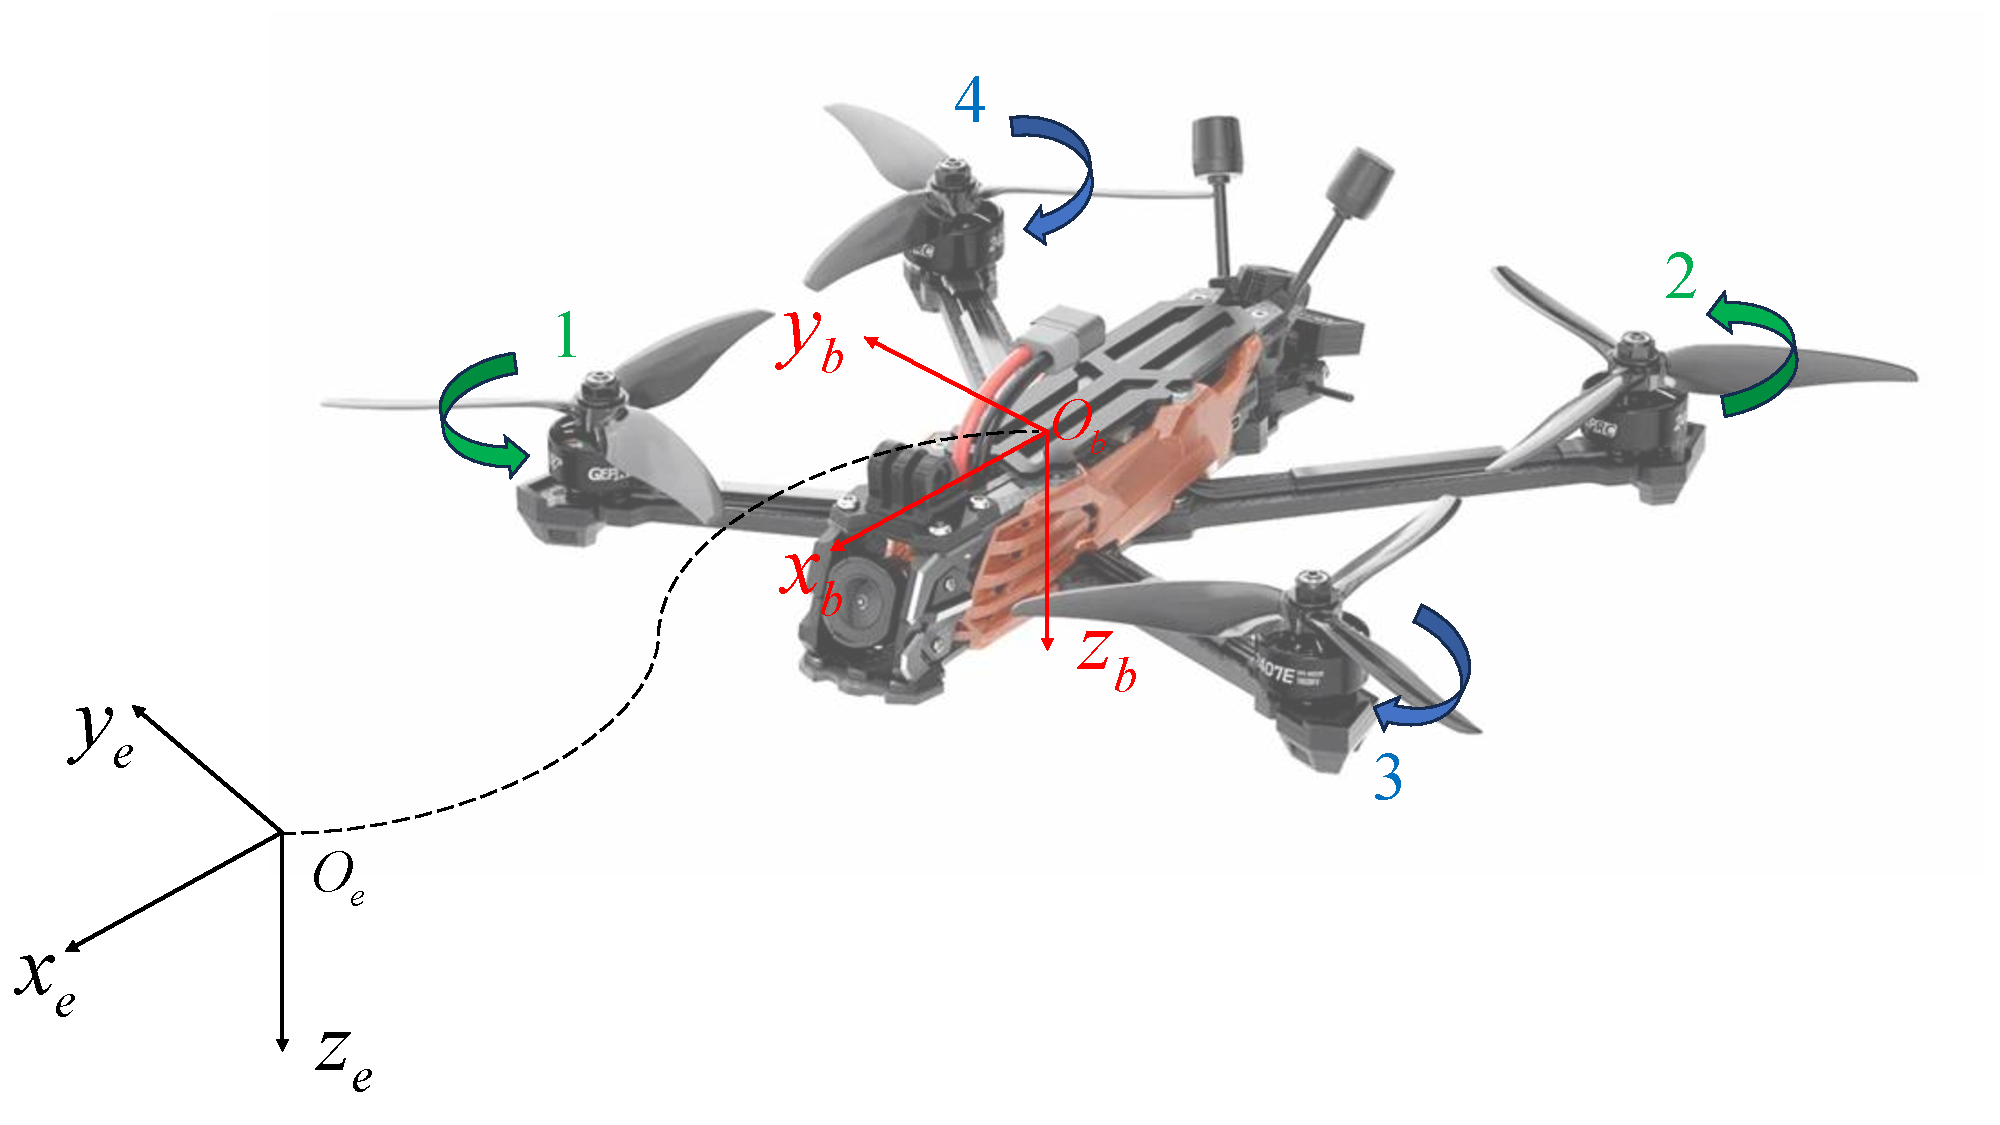
\includegraphics[width=8cm]{Image/fig1.pdf}}
\vskip2mm
{\small 图1\quad 四旋翼模型与机体/惯性坐标系定义
\\
Fig.\,1\quad Quadrotor model and definition of body/inertial frames}}
\end{center}

设第 $i$ 个旋翼($i=1,2,3,4$)的桨毂中心在机体系下的安装位置为常矢量
$\bm{r}_i\in\mathbb{R}^3$, 桨盘法向单位矢量取为升力正方向, 对于共面等桨距布局有
$\bm{n}_i=[0,\ 0,\ -1]^{\mathrm{T}}$.
以 $\sigma_i=\pm 1$ 表示旋翼转向, $\sigma_i=+1$ 表示旋翼角速度沿 $+\bm{n}_i$ 方向;
以 $\Omega_i>0$ 表示旋翼转速, $\psi_i$ 表示桨叶方位角(在桨盘平面内自 $\bm{x}_b$ 轴量起).
环境风速在惯性系下记为 $\bm{v}_w$.

\subsection{桨毂运动学与相对来流分解}
\label{subsec:hub_kinematics}

由于旋翼与机体固连, 在机体系下有 $\dot{\bm{r}}_i\equiv\bm{0}$, 故第 $i$ 个旋翼桨毂
在惯性系下的位置、速度与加速度分别为
\begin{align}
\bm{p}_i&=\bm{p}+\bm{R}\,\bm{r}_i \label{eq:hub_p}\\[2pt]
\bm{v}_i&=\bm{v}+\bm{R}\left(\bm{\omega}\times\bm{r}_i\right) \label{eq:hub_v}\\[2pt]
\bm{a}_i&=\bm{a}+\bm{R}\left[\dot{\bm{\omega}}\times\bm{r}_i
+\bm{\omega}\times\left(\bm{\omega}\times\bm{r}_i\right)\right] \label{eq:hub_a}
\end{align}
% 需要核对,切向加速度是什么方向,向心加速度是什么方向
式~(\ref{eq:hub_a}) 中,\(\dot{\bm\omega}\times\bm r_i\) 为机体角速度变化产生的Euler加速度;当机体转轴方向固定时,该项表现为绕转轴运动的切向加速度.\(\bm\omega\times(\bm\omega\times\bm r_i)\) 为向心加速度,其方向由桨毂指向机体瞬时转轴;二者共同构成旋翼所承受的附加过载.

在明确桨毂自身的刚体运动之后, 进一步计入环境风的影响, 考察桨毂相对气流的运动状态.计入环境风后, 桨毂中心相对于空气的速度在机体系下表示为

\begin{equation}
\bm{u}_i=\bm{R}^{\mathrm{T}}\left(\bm{v}-\bm{v}_w\right)+\bm{\omega}\times\bm{r}_i
\label{eq:u_hub}
\end{equation}

将 $\bm{u}_i$ 沿桨盘法向与桨盘平面内分解, 得到轴向来流速度与面内(侧向)来流速度

\begin{equation}
V_{a,i}=\bm{u}_i^{\mathrm{T}}\bm{n}_i,\qquad
V_{t,i}=\left\|\left(\bm{I}_3-\bm{n}_i\bm{n}_i^{\mathrm{T}}\right)\bm{u}_i\right\|
\label{eq:decompose}
\end{equation}

其中 $V_{a,i}$ 以爬升方向为正.相应地,来流倾角(即来流方向与桨盘法向的夹角)与来流方位角定义为

\begin{equation}
\begin{aligned}
\alpha_{p,i}&=\operatorname{atan2}\!\left(V_{t,i},V_{a,i}\right), \\
\psi_{w,i}&=\operatorname{atan2}\!\left(u_{i,y},\ u_{i,x}\right)
\end{aligned}
\label{eq:alpha_psiw}
\end{equation}

设桨半径为 $R_p$, 定义前进比与轴向入流比

\begin{equation}
\mu_i=\frac{V_{t,i}}{\Omega_i R_p},\qquad
\lambda_{c,i}=\frac{V_{a,i}}{\Omega_i R_p}
\label{eq:mu_lambda}
\end{equation}

诱导入流比 $\lambda_{\mathrm{ind},i}$ 由 Glauert 前飞动量定理[11]确定, 尾迹偏斜角为 $\chi_i$:

\begin{equation}
\begin{aligned}
\lambda_{\mathrm{ind},i}&=\lambda_{c,i}+\frac{C_T}{2\sqrt{\mu_i^2+\lambda_{\mathrm{ind},i}^2}}, \\
\chi_i&=\arctan\frac{\mu_i}{\lambda_{c,i}+\lambda_{\mathrm{ind},i}}
\end{aligned}
\label{eq:glauert}
\end{equation}

式中 $C_T=T_i/\left(\rho_\infty\pi R_p^2(\Omega_i R_p)^2\right)$ 为基于桨尖速度的旋翼拉力系数,
其中$T_i$ 由第~\ref{subsec:lift}~节式~(\ref{eq:thrust}) 的叶素积分给出,$\rho_\infty$ 为空气密度.
\end{multicols}%开始通栏显示
\begin{center}
\vbox{
\centerline{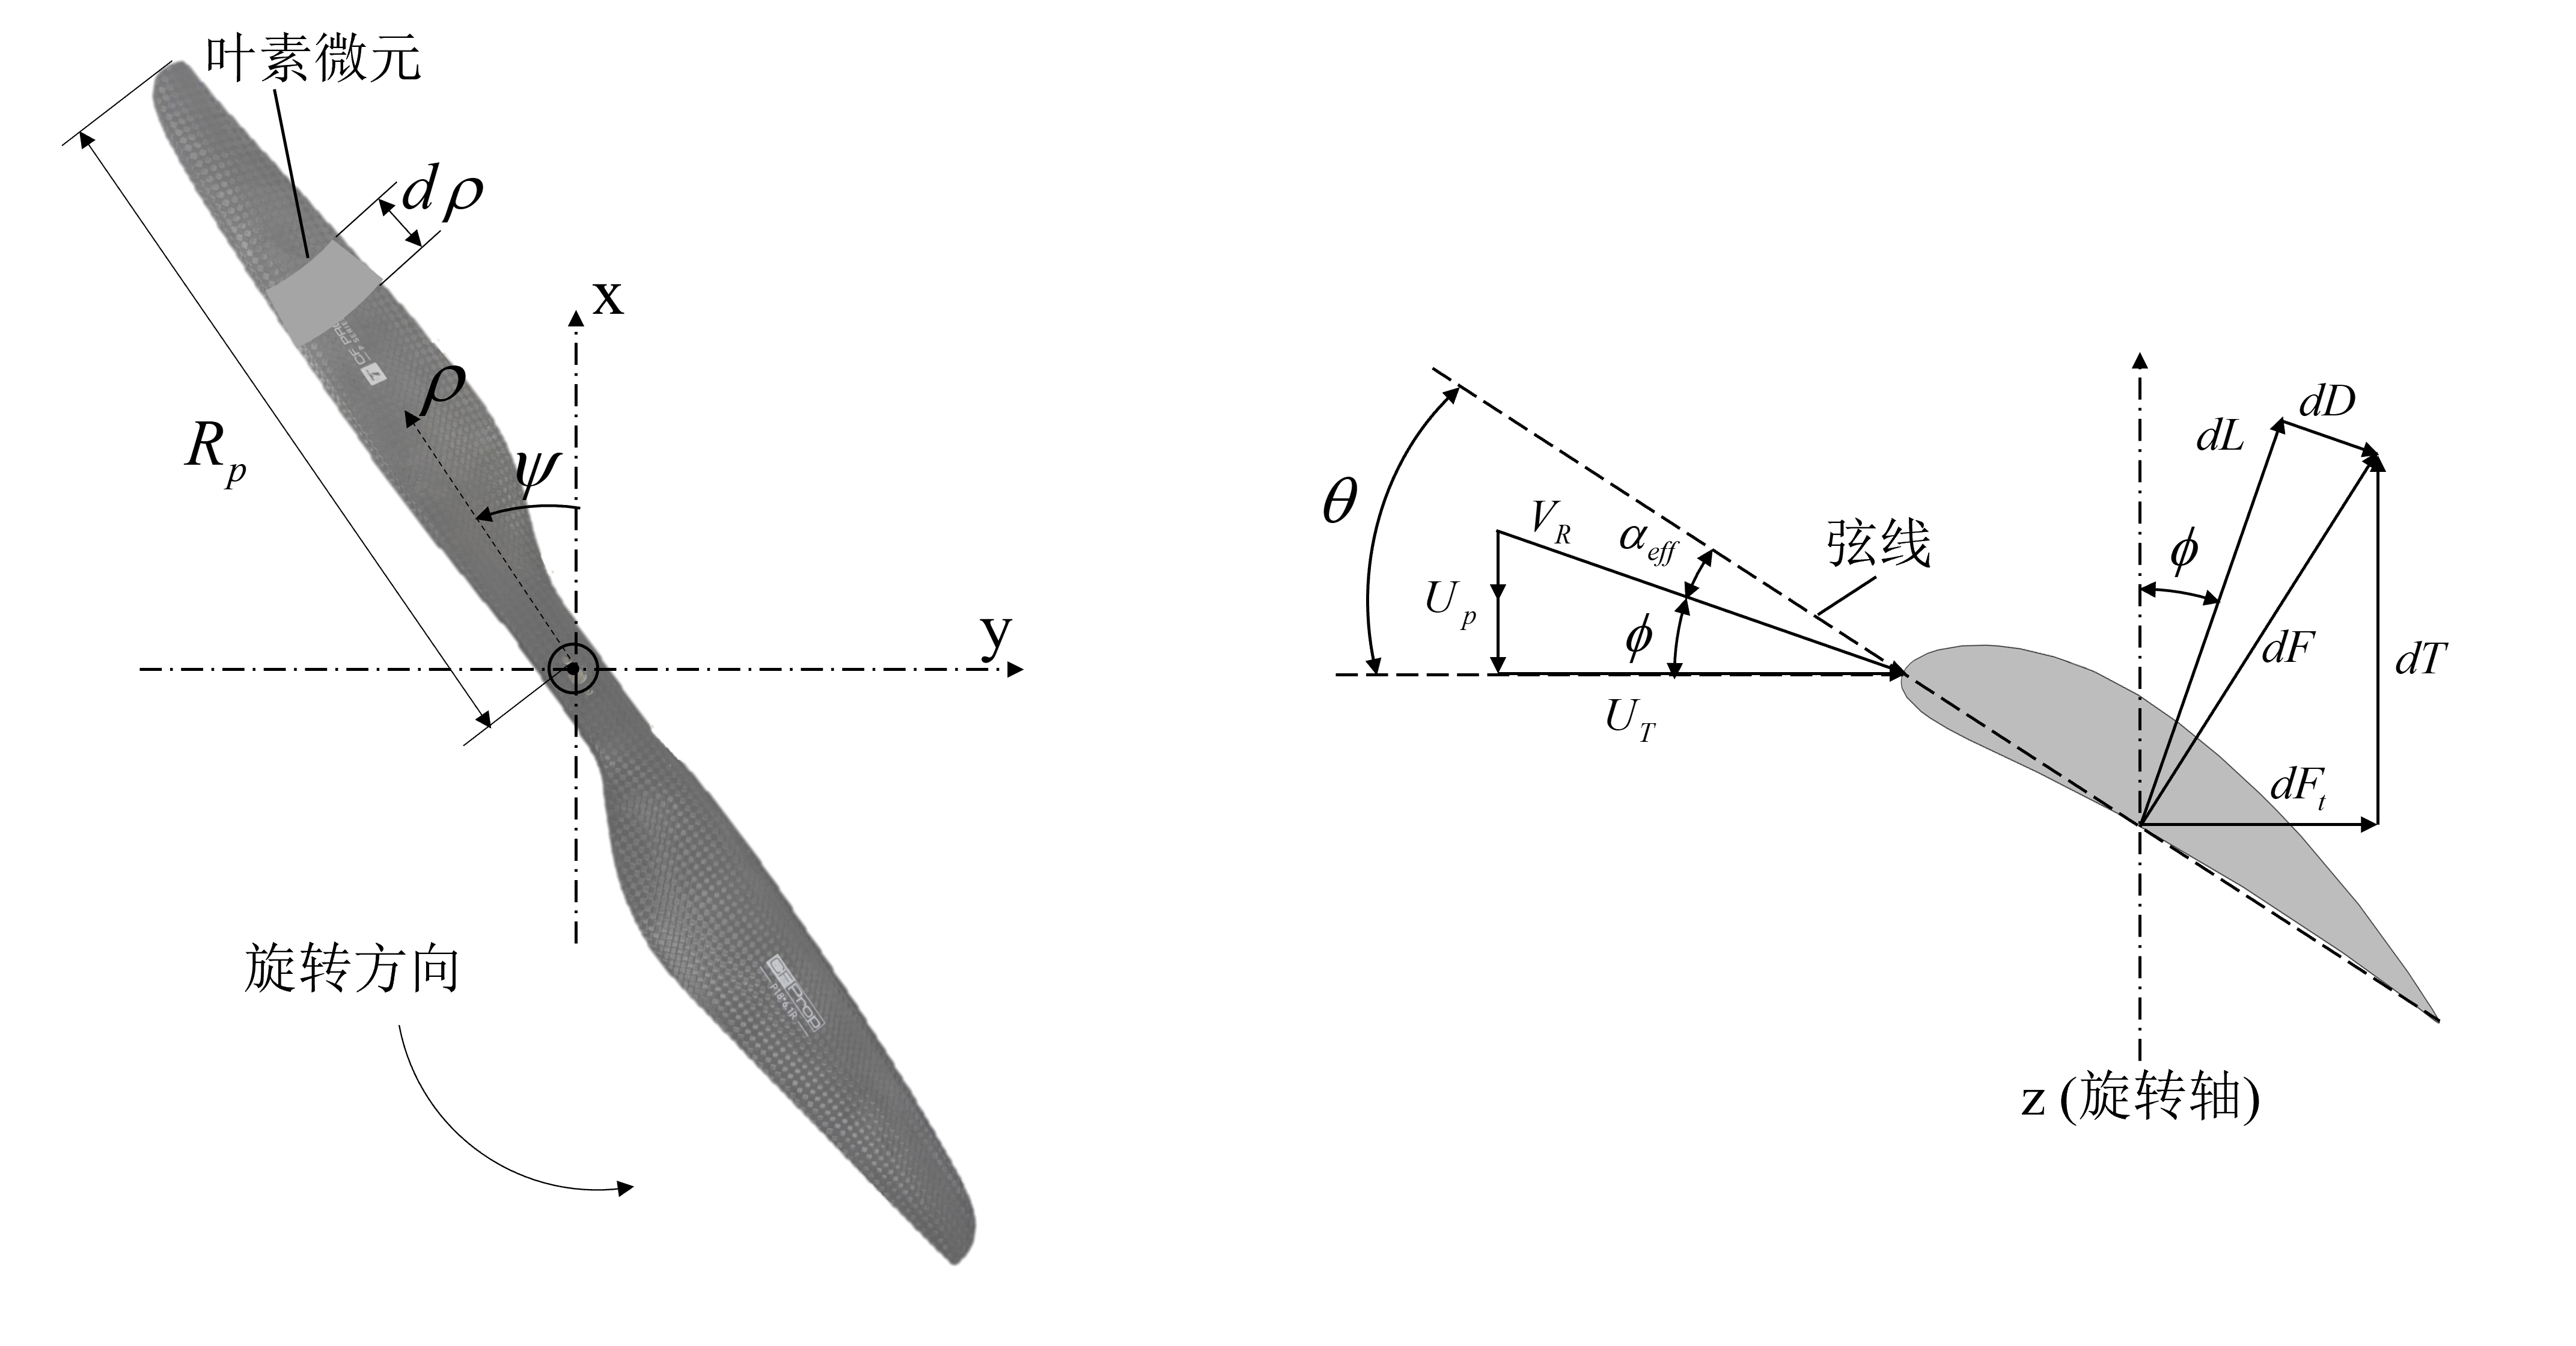
\includegraphics[width=15cm]{Image/fig2.png}}
\vskip2mm
{\small 图2\quad 旋翼坐标、叶素离散及局部来流与气动力分解
\\
Fig.\,2\quad Rotor coordinates, blade element discretization and decomposition of local inflow and aerodynamic forces}}
\end{center}
\begin{multicols}{2}%开始双栏显示
\subsection{叶素气动力建模}
\label{subsec:rotation}
\label{subsec:blade_element}

如图2所示, 对位于展向位置 $\rho\in[\rho_0,\ R_p]$、方位角 $\psi$ 处的叶素, 综合
式~(\ref{eq:u_hub})$\sim$式~(\ref{eq:glauert}), 其相对空气的切向速度与法向速度为

\begin{align}
U_T(\rho,\psi)&=\Omega_i\rho+\sigma_i V_{t,i}\sin\!\left(\psi-\psi_{w,i}\right) \label{eq:UT}\\[2pt]
U_P(\rho,\psi)&=V_{a,i}+v_{\mathrm{ind}}(\rho,\psi) \label{eq:UP}
\end{align}
式~(\ref{eq:UT}) 中的 $\sigma_i V_{t,i}\sin(\psi-\psi_{w,i})$ 项反映了侧向来流
造成的前行桨叶与后行桨叶的动压不对称; $v_{\mathrm{ind}}(\rho,\psi)$
为诱导入流速度.

由式~(\ref{eq:UT}) 和式~(\ref{eq:UP}) 可得叶素处的入流角与有效迎角

\begin{equation}
\begin{aligned}
\phi(\rho,\psi)&=\arctan\frac{U_P}{U_T},\\
\alpha_{\mathrm{eff}}(\rho,\psi)&=\theta(\rho)-\phi(\rho,\psi)
\end{aligned}
\label{eq:aoa}
\end{equation}

其中 $\theta(\rho)$ 为由摄影测量获得的无载桨叶安装角分布,本文采用刚性桨叶近似. 

\label{subsec:induced}

式~(\ref{eq:UP}) 中的诱导速度 $v_{\mathrm{ind}}$ 无法直接测量, 需要建模确定.
在轴向来流下, 诱导速度在桨盘内近似均匀; 而在斜来流下, 尾迹发生偏斜,
诱导速度沿桨盘呈现前行--后行方向(纵向)的非均匀分布. 本文采用 Serrano 等验证的
一阶谐波线性入流模型[9], 将局部诱导入流比表示为平均诱导入流比与纵向一阶谐波之和:

\begin{equation}
\begin{aligned}
v_{\mathrm{ind}}(\rho,\psi)&=\lambda_{\mathrm{ind}}(\rho,\psi)\,\Omega_{i}R_p,\\
\lambda_{\mathrm{ind}}(\rho,\psi)&=\lambda_{\mathrm{ind},i}\left[1+k_x\frac{\rho}{R_p}\sin\!\left(\psi-\psi_{w,i}\right)\right]
\end{aligned}
\label{eq:ind_vel}
\end{equation}

式中 $\lambda_{\mathrm{ind},i}$ 为由式~(\ref{eq:glauert}) 隐式确定的平均诱导入流比,
$k_x$ 为纵向入流梯度系数, 其大小随尾迹偏斜角 $\chi_i$ 增大而增大;
当来流趋于轴向($\mu_i\to0$)时 $k_x\to0$, 式~(\ref{eq:ind_vel}) 退化为均匀入流.
由于 $\lambda_{\mathrm{ind},i}$ 依赖于旋翼拉力系数 $C_T$(本身即待求量),
式~(\ref{eq:glauert})--式~(\ref{eq:thrust}) 构成耦合系统, 需通过固定点迭代求解:
先给定静态环境下悬停时的 $C_T$ 初值求解 $\lambda_{\mathrm{ind},i}$ 与 $v_{\mathrm{ind}}$,
再由叶素积分更新 $C_T$, 迭代至收敛.

\label{subsec:lift}

在得到局部速度场与诱导速度后, 叶素气动力由二维翼型极线查表获得. 对展向位置
$\rho$、方位角 $\psi$ 处的叶素, 其局部合速度为 $V_R=\sqrt{U_T^2+U_P^2}$,
当地雷诺数为

\begin{equation}
Re(\rho,\psi)=\frac{\rho_\infty c(\rho)\,V_R}{\mu_\infty}
\label{eq:Re}
\end{equation}

其中 $c(\rho)$ 为弦长分布, $\mu_\infty$为动力粘度.
以有效迎角 $\alpha_{\mathrm{eff}}$ 与雷诺数 $Re$ 查取由 XFOIL[12] 计算的翼型极曲线
$C_l(\alpha_{\mathrm{eff}},Re)$、$C_d(\alpha_{\mathrm{eff}},Re)$, 得叶素单位展长的
升力与阻力

\begin{equation}
\begin{aligned}
\mathrm{d}L&=\frac{1}{2}\rho_\infty V_R^2 C_l\,c(\rho)\,\mathrm{d}\rho,\\
\mathrm{d}D&=\frac{1}{2}\rho_\infty V_R^2 C_d\,c(\rho)\,\mathrm{d}\rho
\end{aligned}
\label{eq:dLdD}
\end{equation}

将 $\mathrm{d}L$、$\mathrm{d}D$ 投影至旋翼轴线方向, 得叶素对轴向升力的贡献

\begin{equation}
\mathrm{d}T=\mathrm{d}L\cos\phi-\mathrm{d}D\sin\phi
\label{eq:dT}
\end{equation}

沿有效展向区间 $[\rho_0,\ R_p]$ 与完整方位角 $[0,\ 2\pi]$ 积分, 并计入桨叶片数
$N_b$, 即得旋翼的轴向升力

\begin{equation}
T_i=\frac{N_b}{2\pi}\int_{0}^{2\pi}\!\!\int_{\rho_0}^{R_p}
\mathrm{d}T\mathrm{d}\rho\,\mathrm{d}\psi
\label{eq:thrust}
\end{equation}

综上, 当无人机运动时, 影响任一旋翼产生升力的变量可以归约为:
\begin{equation}
\bm{s}_i^{\mathrm{aero}}=\left\{V_{a,i},\ V_{t,i},\ \psi_{w,i}, \ \Omega_i\right\}
\label{eq:state_aero}
\end{equation}
于是旋翼轴向升力可表示为 $T_i=f\!\left(\bm{s}_i^{\mathrm{aero}}\right)$.其中$V_{a,i},\ V_{t,i},\ \psi_{w,i}$共同描述来流速度和倾角,而$\Omega_i$描述旋翼转速.

\section{控制架构}
\label{sec:control}

\subsection{传统控制架构及其局限性}
\label{subsec:conventional}

四旋翼无人机飞行控制器由位置-速度外环、姿态-角速度内环与控制分配器组成.外环根据位置与速度误差生成期望总升力 $T$ 与期望姿态 $\bm{\theta}_d$,内环生成期望控制力矩 $\bm{M}=[\tau_x,\tau_y,\tau_z]^{\mathrm{T}}$;控制分配器进一步将期望总升力与力矩分解为各旋翼的目标升力 $T_{d,i}$.随后,升力-控制量映射器将 $T_{d,i}$ 转换为归一化电机指令 $u_i$,再由电子调速器、电机与螺旋桨产生实际升力 $T_i$.该结构如图3(a)所示.

如图3(b)所示,在现有开源飞控系统中[13],升力-控制量映射器通常定义为如下的静态二次映射:
\begin{equation}
T_{d,i}=f_{map}(u_i)=c_a u_i^2+(1-c_a)u_i
\label{eq:static_map}
\end{equation}
其中,$c_a\in[0,1]$ 为无人机悬停时标定的固定参数,用于描述旋翼升力与转速之间的近似平方关系.
在近悬停和缓慢姿态变化条件下,式~(\ref{eq:static_map})能够满足常规控制需求;当局部来流发生显著变化时,相同控制量对应的实际升力将随工况改变,导致期望升力与实际升力之间产生系统性偏差.由于传统架构缺少旋翼升力反馈,该偏差只能通过外层姿态或位置误差间接修正,控制作用链路较长,并可能在强扰动或快速机动时引起超调和振荡.

\subsection{升力闭环控制架构}
\label{subsec:closed_loop}

为使控制系统直接感知执行器层面的实际作用力,本文在控制分配器之后增设独立的旋翼升力内环,该内环由前馈控制器与反馈补偿器两部分组成,如图3(c)所示.
前馈控制器包含旋翼升力逆模型与转速-控制量映射器.给定期望升力 $T_{d,i}$ 后,旋翼升力逆模型依据当前来流速度和来流倾角求解所需的前馈转速 $\Omega_{\mathrm{d,i}}$,再经静态标定的转速-控制量映射转换为前馈控制量 $u_{\mathrm{ff,i}}$.
前馈量已涵盖高机动工况下的来流速度与桨盘姿态信息,但电池压降、旋翼间气动干扰等未建模误差仍会造成升力偏差,故引入反馈补偿器予以校正.反馈补偿器以期望升力 $T_{d,i}$ 与同轴力传感器实测升力 $T_i$ 之差为输入,生成控制修正量$u_{\mathrm{fb,i}}$,与前馈控制量叠加得到总输出 $u_{\mathrm{c,i}}=u_{\mathrm{ff,i}}+u_{\mathrm{fb,i}}$.

\end{multicols}%开始通栏显示
\begin{center}
\vbox{
\centerline{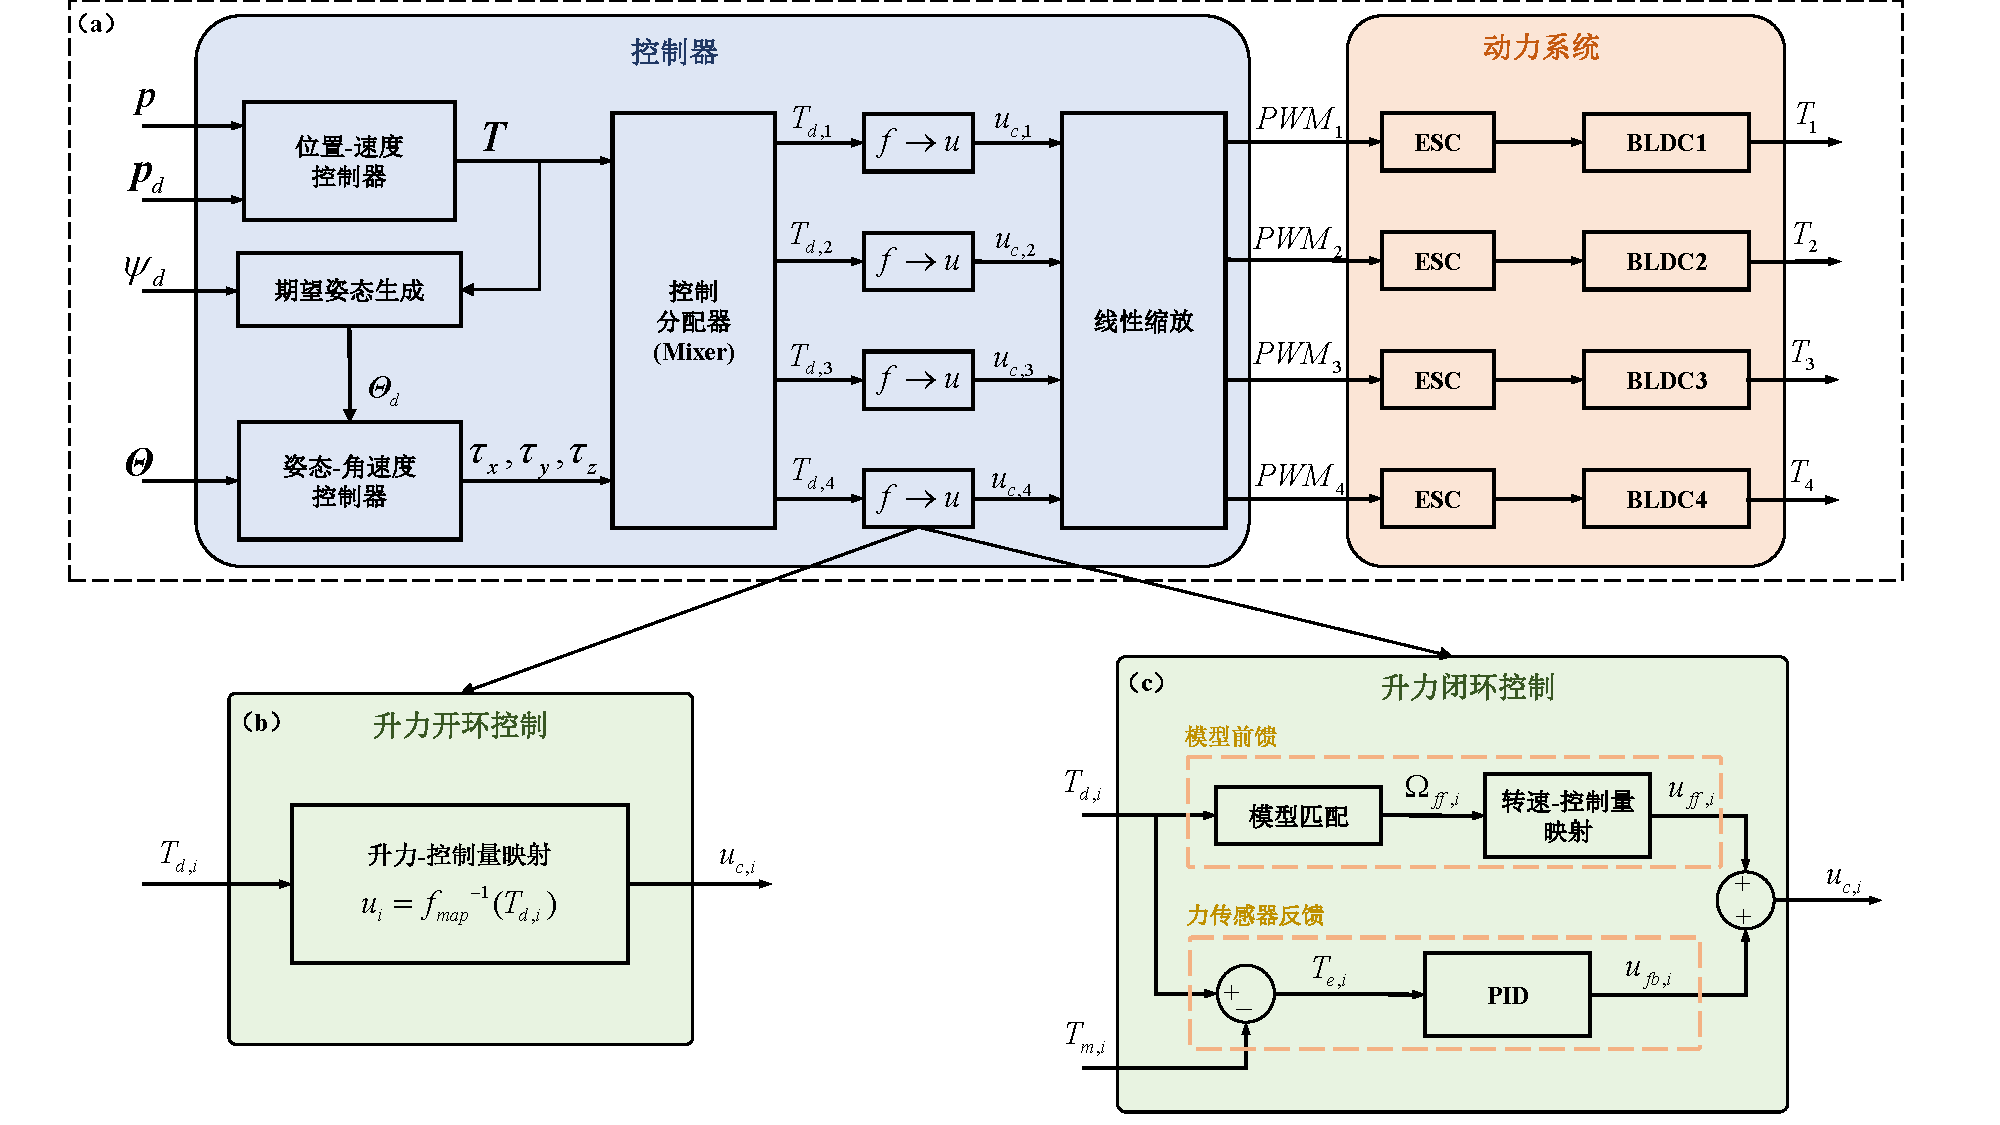
\includegraphics[width=15cm]{Image/fig3.pdf}}
\vskip2mm
{\small 图3\quad 四旋翼无人机控制架构;(a)总体控制架构;(b)传统升力开环控制架构;(c)升力闭环控制架构
\\
Fig.\,3\quad Control Architecture for Quadcopter UAVs; (a) Overall Control Architecture; (b) Conventional Open-Loop thrust Control Architecture; (c) Closed-Loop thrust Control Architecture}}
\end{center}
\begin{multicols}{2}%开始双栏显示

\begin{center}
\vbox{
\centerline{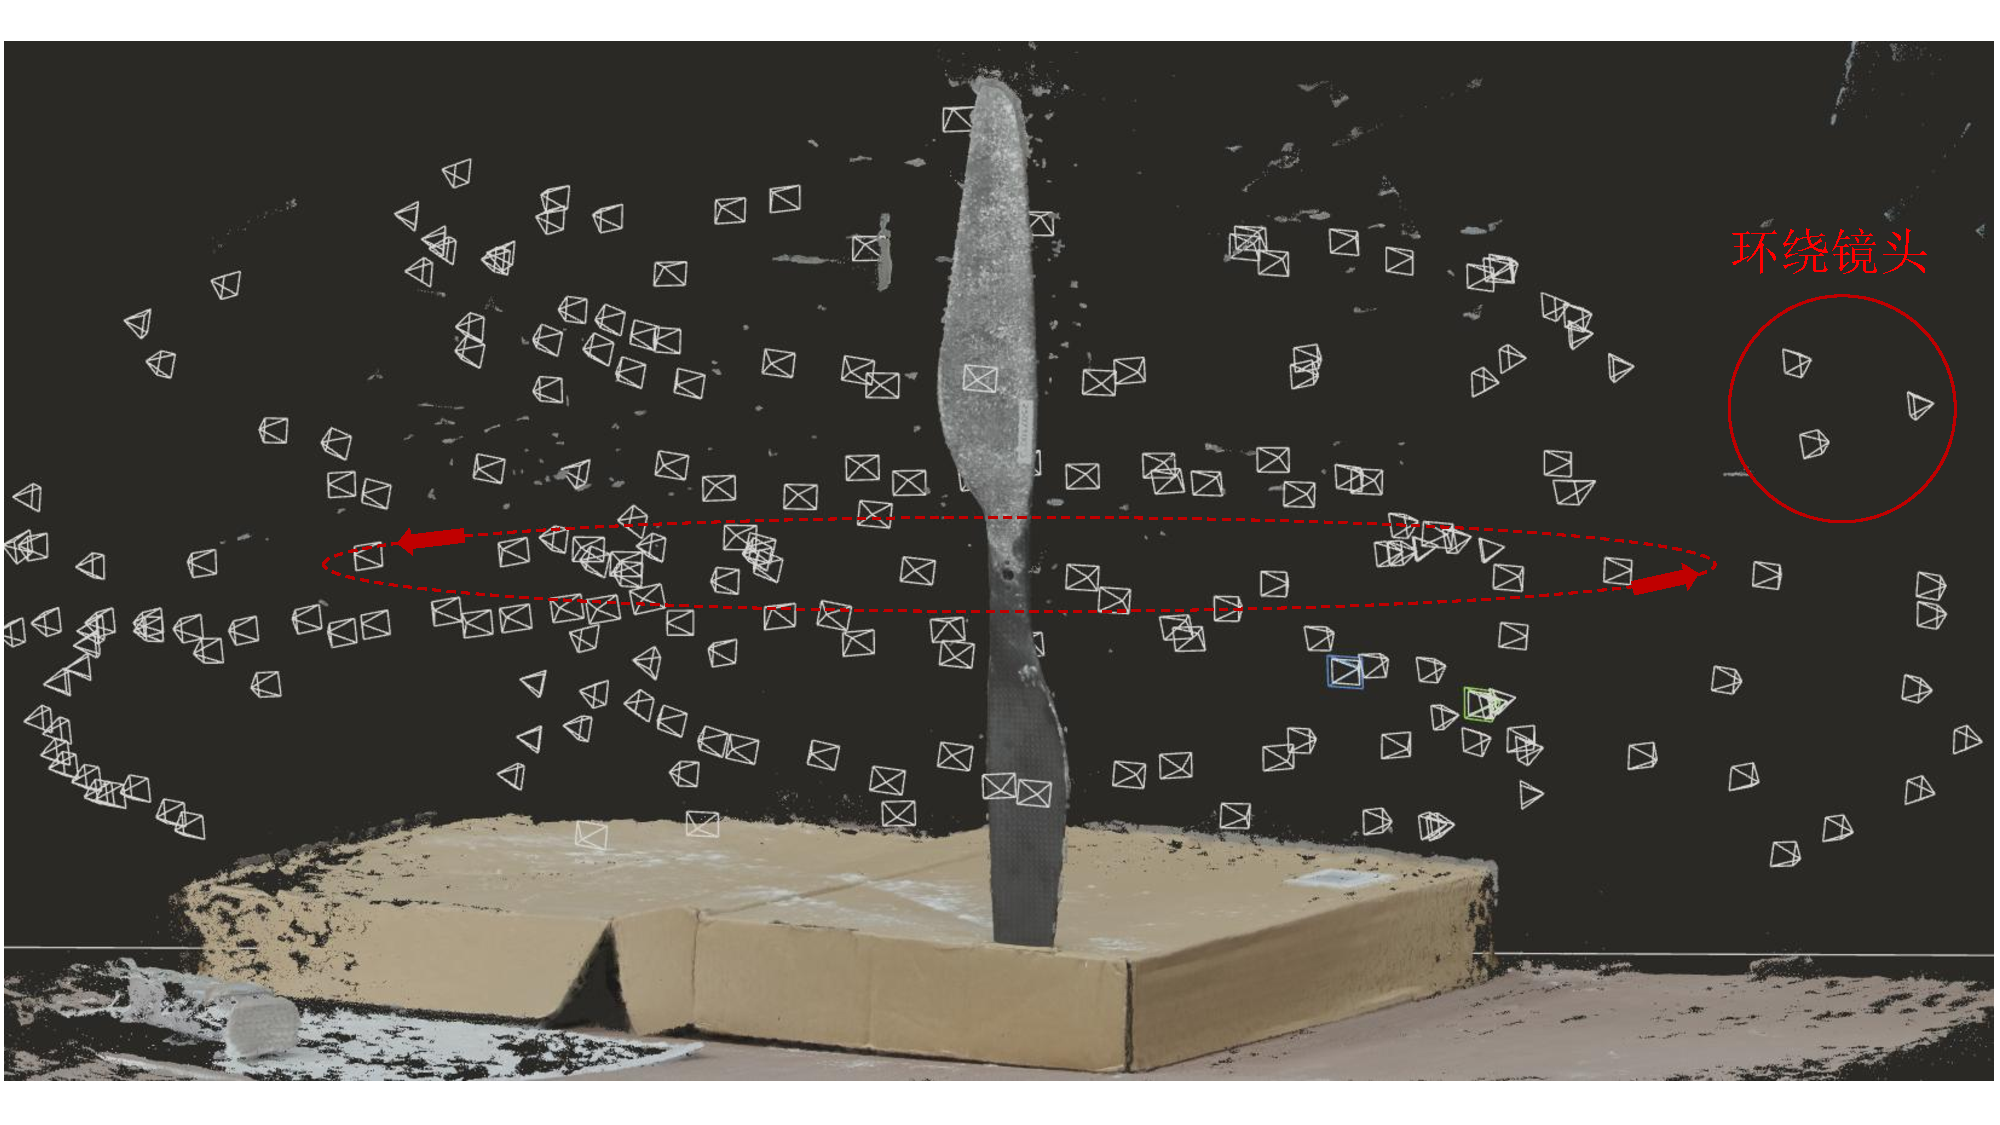
\includegraphics[width=8cm]{Image/fig4a.pdf}}
{\small (a)}
\centerline{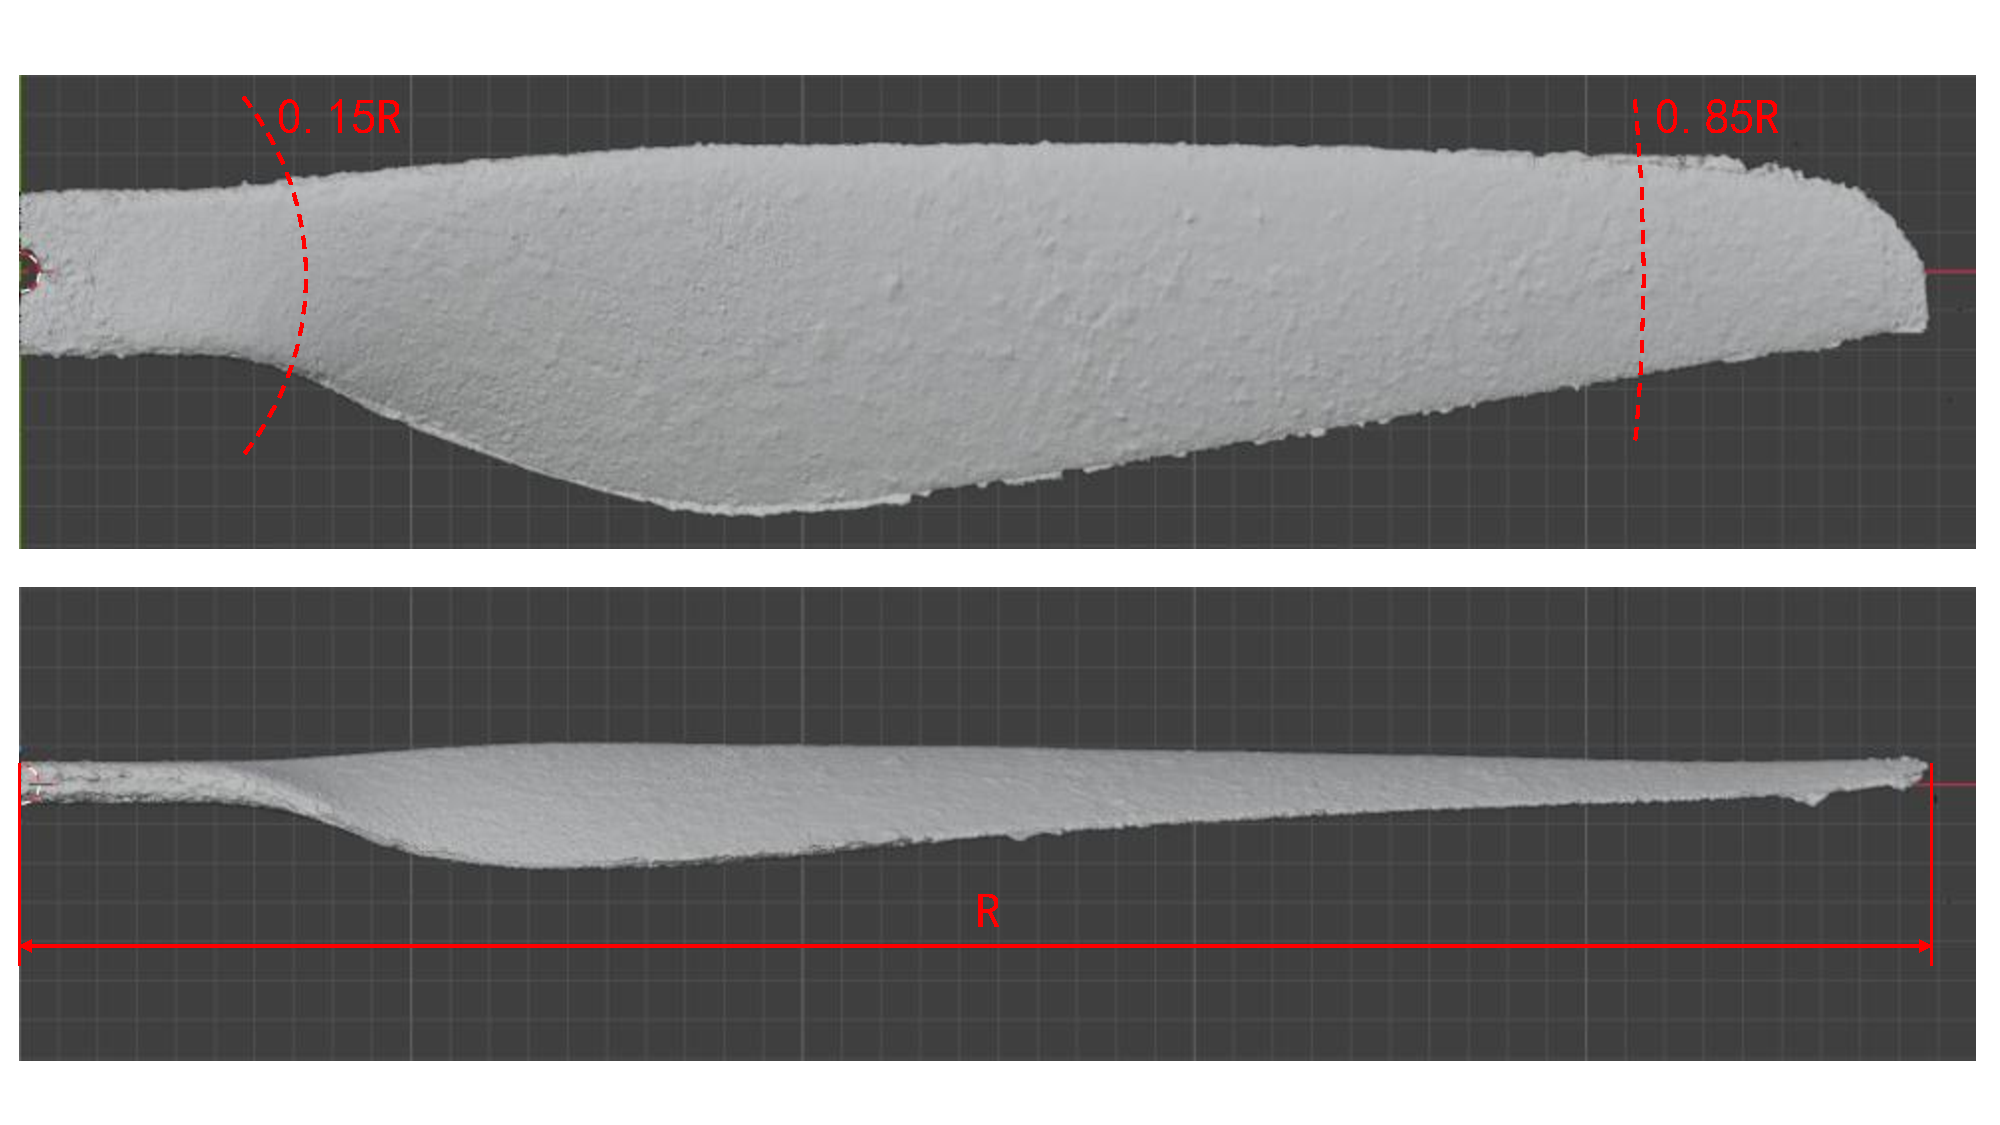
\includegraphics[width=8cm]{Image/fig4b.pdf}}
{\small (b)}
\vskip2mm
{\small 图4\quad 螺旋桨摄影测量、三维重建与截面提取过程;(a)螺旋桨三维重建;(b)截面提取
\\
Fig.\,4\quad Photogrammetry, 3D reconstruction and cross-section extraction of the propeller;(a)3D reconstruction of the propeller;(b)Cross-section extraction}}
\end{center}

\section{实施}
本节介绍上述理论方法从理论到实现的完整工程链条。首先为了离线完整计算叶素理论,通过摄影测量提取桨叶几何与翼型气动数据;随后搭建了模拟高机动飞行工况的旋转式单旋翼测试台,并介绍了升力测量单元的结构细节和传感器标定方法;最后将升力闭环控制架构部署于实际飞控,并介绍了转速-控制量静态标定方法.在实施过程中,部署于飞控的升力模型前馈无需升力试验数据进行修正,只需要摄影测量得到的桨叶几何参数,以及静态标定转速-控制量映射即可.
\subsection{桨叶几何与翼型气动数据获取}
\label{subsec:geo}
叶素模型需要两类输入:一类是弦长$c(\rho)$、安装角$\theta(\rho)$及翼型轮廓随径向位置的变化,另一类是各截面在有效迎角$\alpha_{\mathrm{eff}}$和雷诺数$Re$下的二维气动系数$C_l$、$C_d$.UIUC等公开数据库能够提供部分通用翼型坐标[14],但商业螺旋桨通常只标注直径和标称桨距,缺少上述径向几何及截面数据[15].为此,本文按照摄影测量重建、径向截面提取、二维极线计算的流程获取T-Motor P18$\times$6.1\,CF螺旋桨的模型输入.

三维重建能够将实物的几何信息数字化,其关键在于获取具有稳定尺度和充分表面特征的稠密点云.常用方法可分为激光扫描和摄影测量两类[16]:前者精度较高,但设备成本高昂;后者仅需普通相机即可有效控制成本,但对光照条件较为敏感——物体表面的镜面反光及低纹理区域易导致特征匹配失败、点云产生空洞或局部几何畸变[17].为消除光照的干扰,现有应用通常需要将待重建物体置于背景洁净、光照均匀且无镜面反射的实验室环境中拍摄,这在一定程度上限制了摄影测量在现场或非受控场景下的适用性.

针对碳纤维桨叶表面光泽度高、易产生镜面反光这一特点,本文在拍摄前于桨叶表面均匀撒布一层薄层玉米淀粉,利用其亚光、微粒特性抑制碳纤维表面的镜面反光并引入随机纹理,从源头上降低了摄影测量对光照条件的敏感性.由此,本文无需专业光源和暗室实验室环境,在光照不受控的普通室内环境下完成了螺旋桨的高质量建模.具体地,本文从上、中、下三个高度环绕拍摄,相邻方位的角度间隔不超过$10^{\circ}$,同时补充不同俯仰角下的图像,以保证桨叶各处表面特征均被充分覆盖.照片导入RealityScan后依次完成特征匹配、稠密点云重建和三角网格生成.以桨毂中心为坐标原点,利用实测桨径校准模型尺度,并将模型$z$轴与螺旋桨旋转轴对齐,得到可按无量纲径向位置$r/R$索引的桨叶网格.图4(a)给出了重建点云及相机位姿,图4(b)给出了对齐后的桨叶模型.

三维网格本身不能直接作为叶素模型输入,还需转换为沿展向排列的二维截面.在给定$r/R$处,以同轴圆柱面与桨叶网格求交,将交线展开并投影到局部二维坐标系;识别前、后缘后,分别对上、下表面进行平滑拟合,以减弱点云噪声及网格在尖锐边缘处的畸变.由拟合轮廓计算弦长$c(\rho)$、安装角$\theta(\rho)$和相对厚度$t/c$,再以弦长归一化截面坐标.

摄影测量得到的是无载外形,载荷引起的弹性扭转会改变有效安装角,弯曲会改变局部截面姿态与入流关系,从而影响有效迎角和升力预测.然而弹性变形需要沿桨叶展向的等效弯曲刚度、扭转刚度等结构参数;为简化离线建模流程,本文采用刚性桨叶近似,暂未计入载荷引起的几何变化.

\begin{center}
\vbox{
\centerline{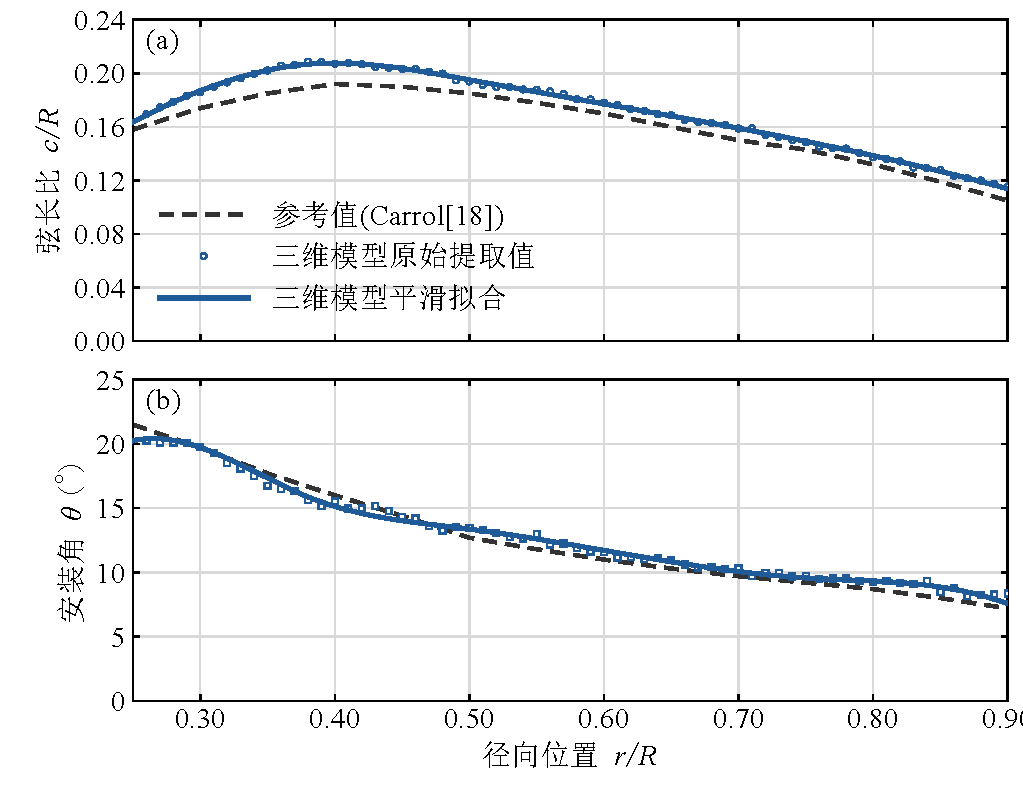
\includegraphics[width=9cm]{Image/fig5_chord_pitch_comparison.pdf}}
\vskip2mm
{\small 图5\quad 桨叶弦长比与安装角的径向分布($0.25\le r/R\le0.90$)
\\
Fig.\,5\quad Radial distributions of blade chord ratio and pitch angle ($0.25\le r/R\le0.90$)}}
\end{center}

为检验几何提取结果,将弦长比$c/R$和安装角$\theta$的径向分布与Carroll[18]基于激光扫描获得的T-Motor 18$\times$6.1桨叶数据进行比较,如图5所示.选取$0.25\le r/R\le0.90$的主要气动承载区间作为比较区间,将两组曲线插值至同一径向网格,并以两者均值作为相对差异的归一化基准.弦长比的平均绝对差异、均方根差异和最大绝对差异分别为0.010、0.011和0.018,平均相对差异为6.0\%;安装角的上述三项绝对差异分别为$0.54^{\circ}$、$0.60^{\circ}$和$1.25^{\circ}$,平均相对差异为4.8\%.两项参数的曲线相关系数均约为0.995,表明摄影测量能够准确描述桨叶的弦长与安装角变化,其几何分辨率满足本文叶素模型的输入要求.

最后,将各径向位置的归一化截面坐标输入XFOIL[12],在覆盖本文叶素工作范围的$\alpha_{\mathrm{eff}}$--$Re$离散网格上计算二维极线,建立供第~\ref{subsec:lift}~节查取的$C_l(\alpha_{\mathrm{eff}},Re)$和$C_d(\alpha_{\mathrm{eff}},Re)$数据库.
\subsection{高机动工况构造:旋翼测试台}
\label{subsec:bench}
为在地面条件下构造可重复的高机动工况,本文搭建旋转悬臂式单旋翼测试平台,如图6(a)所示.驱动电机带动转盘和悬臂绕竖直轴旋转,旋翼单元安装于距离旋转中心$R_0$的悬臂末端上.旋翼单元的细节如图6(b)所示,通过倾转支架与竖直方向的夹角$\theta$,进而调节桨盘攻角$\alpha_p$;通过转台角速度$\Omega_a$改变旋翼单元面对的来流速度.
\begin{center}
\vbox{
\centerline{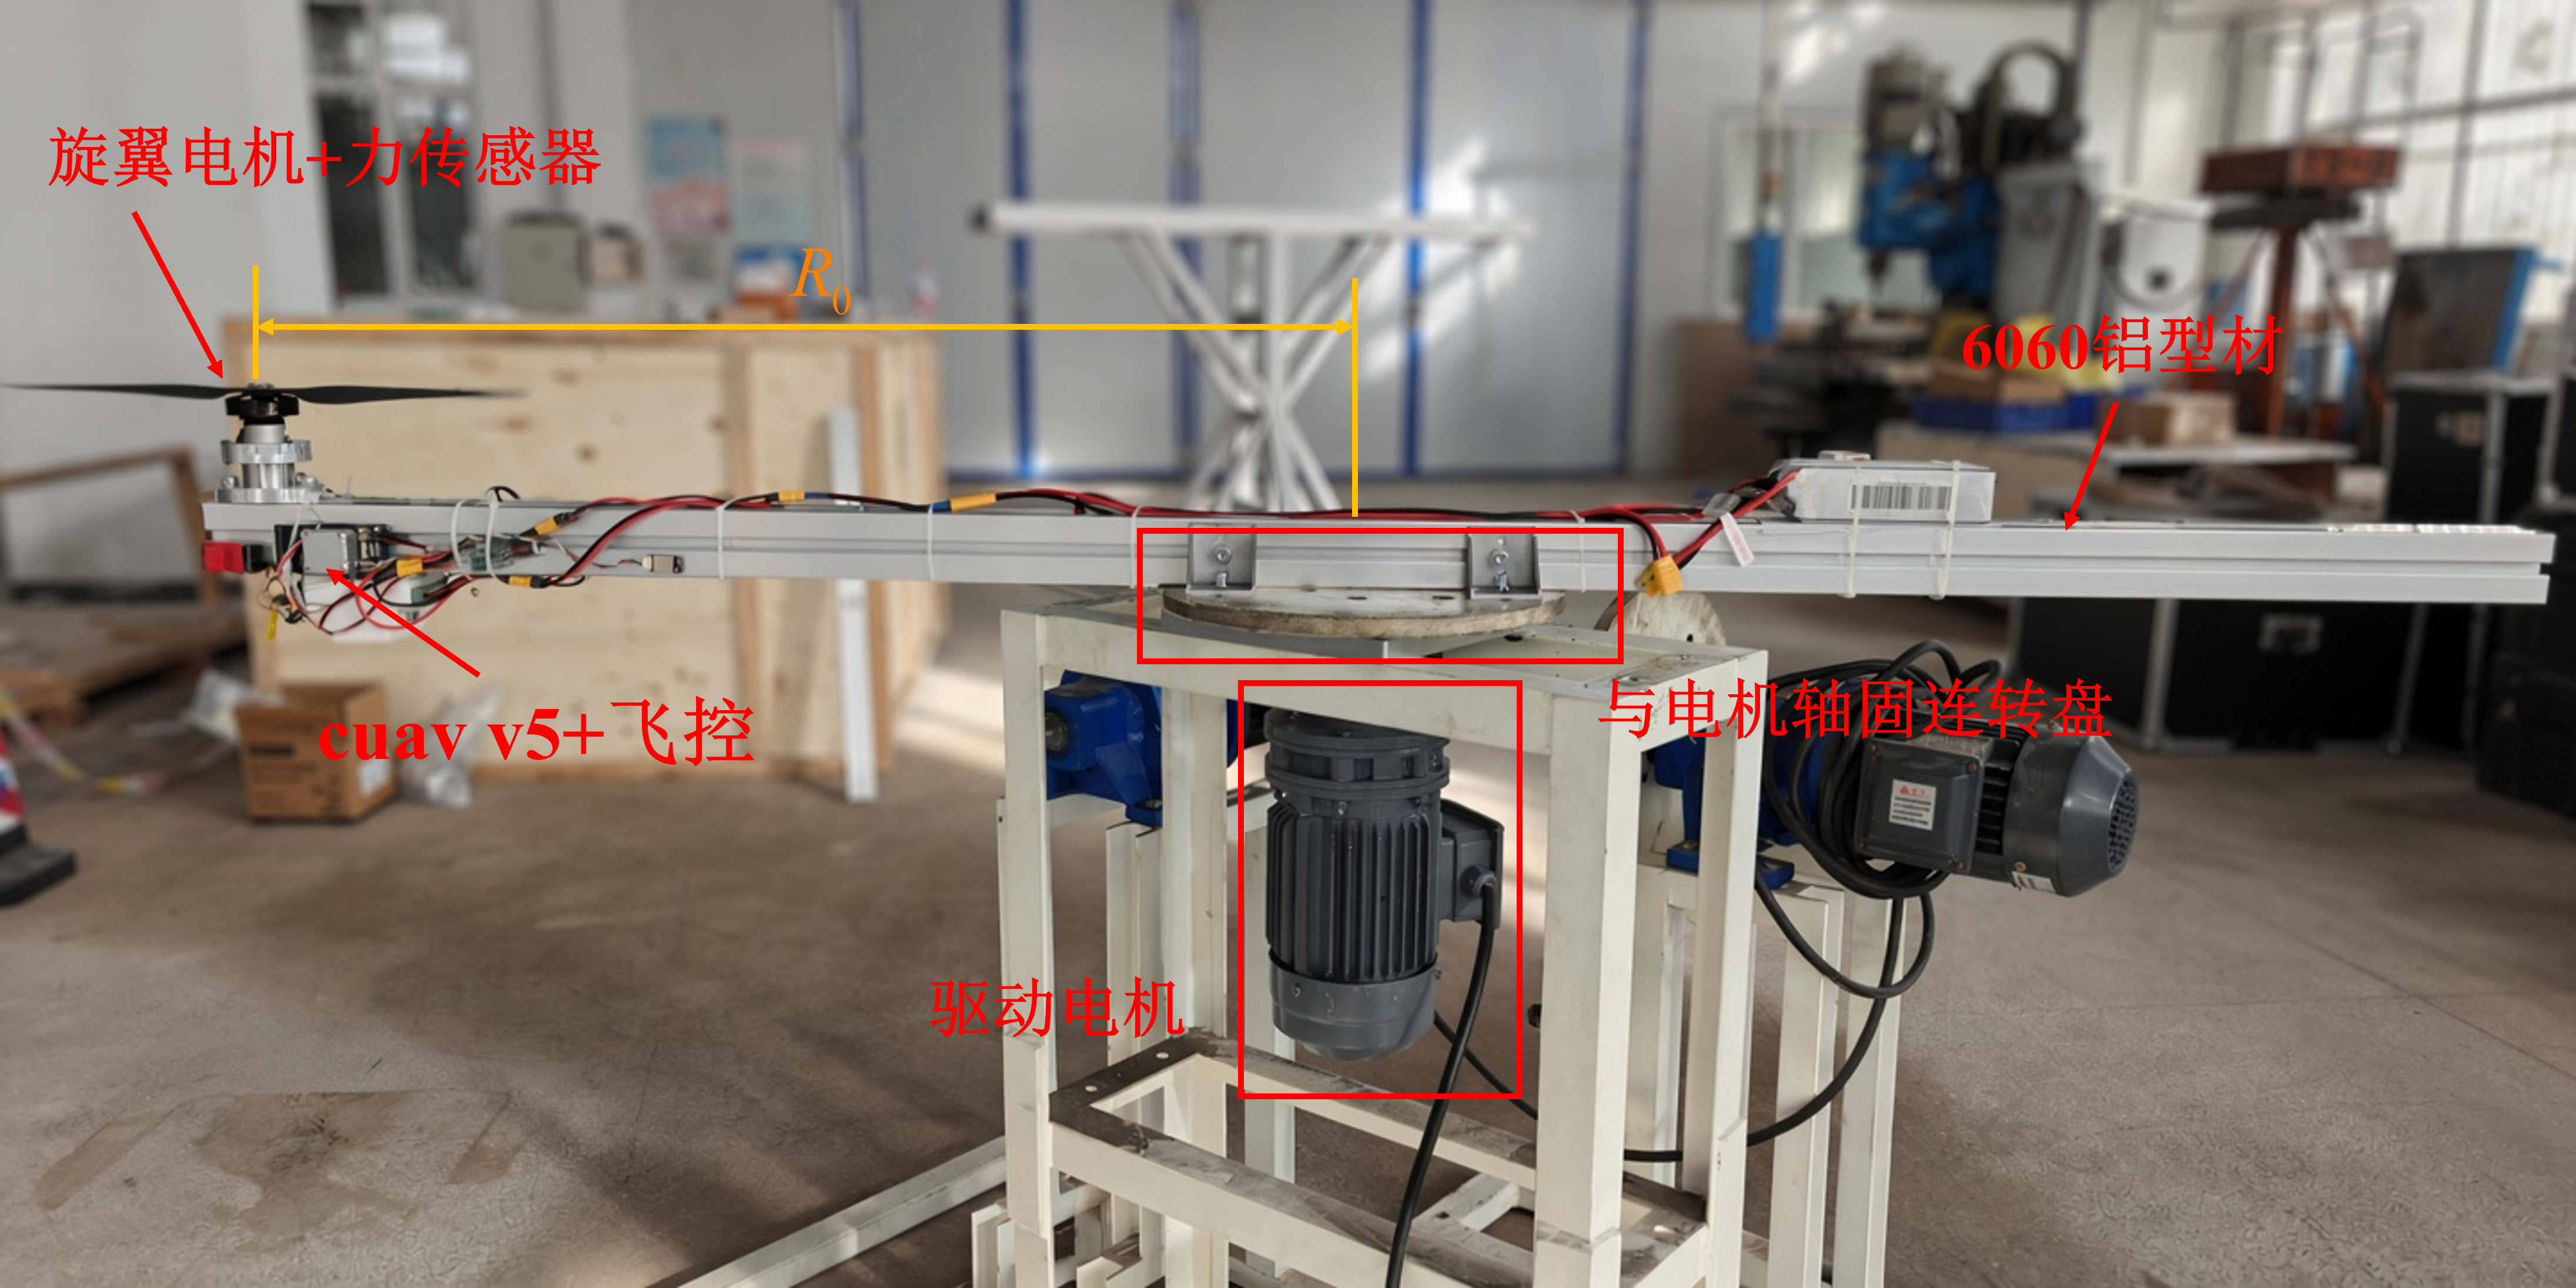
\includegraphics[width=8cm]{Image/图6a-旋转测试台.png}}
{\small (a)}
\centerline{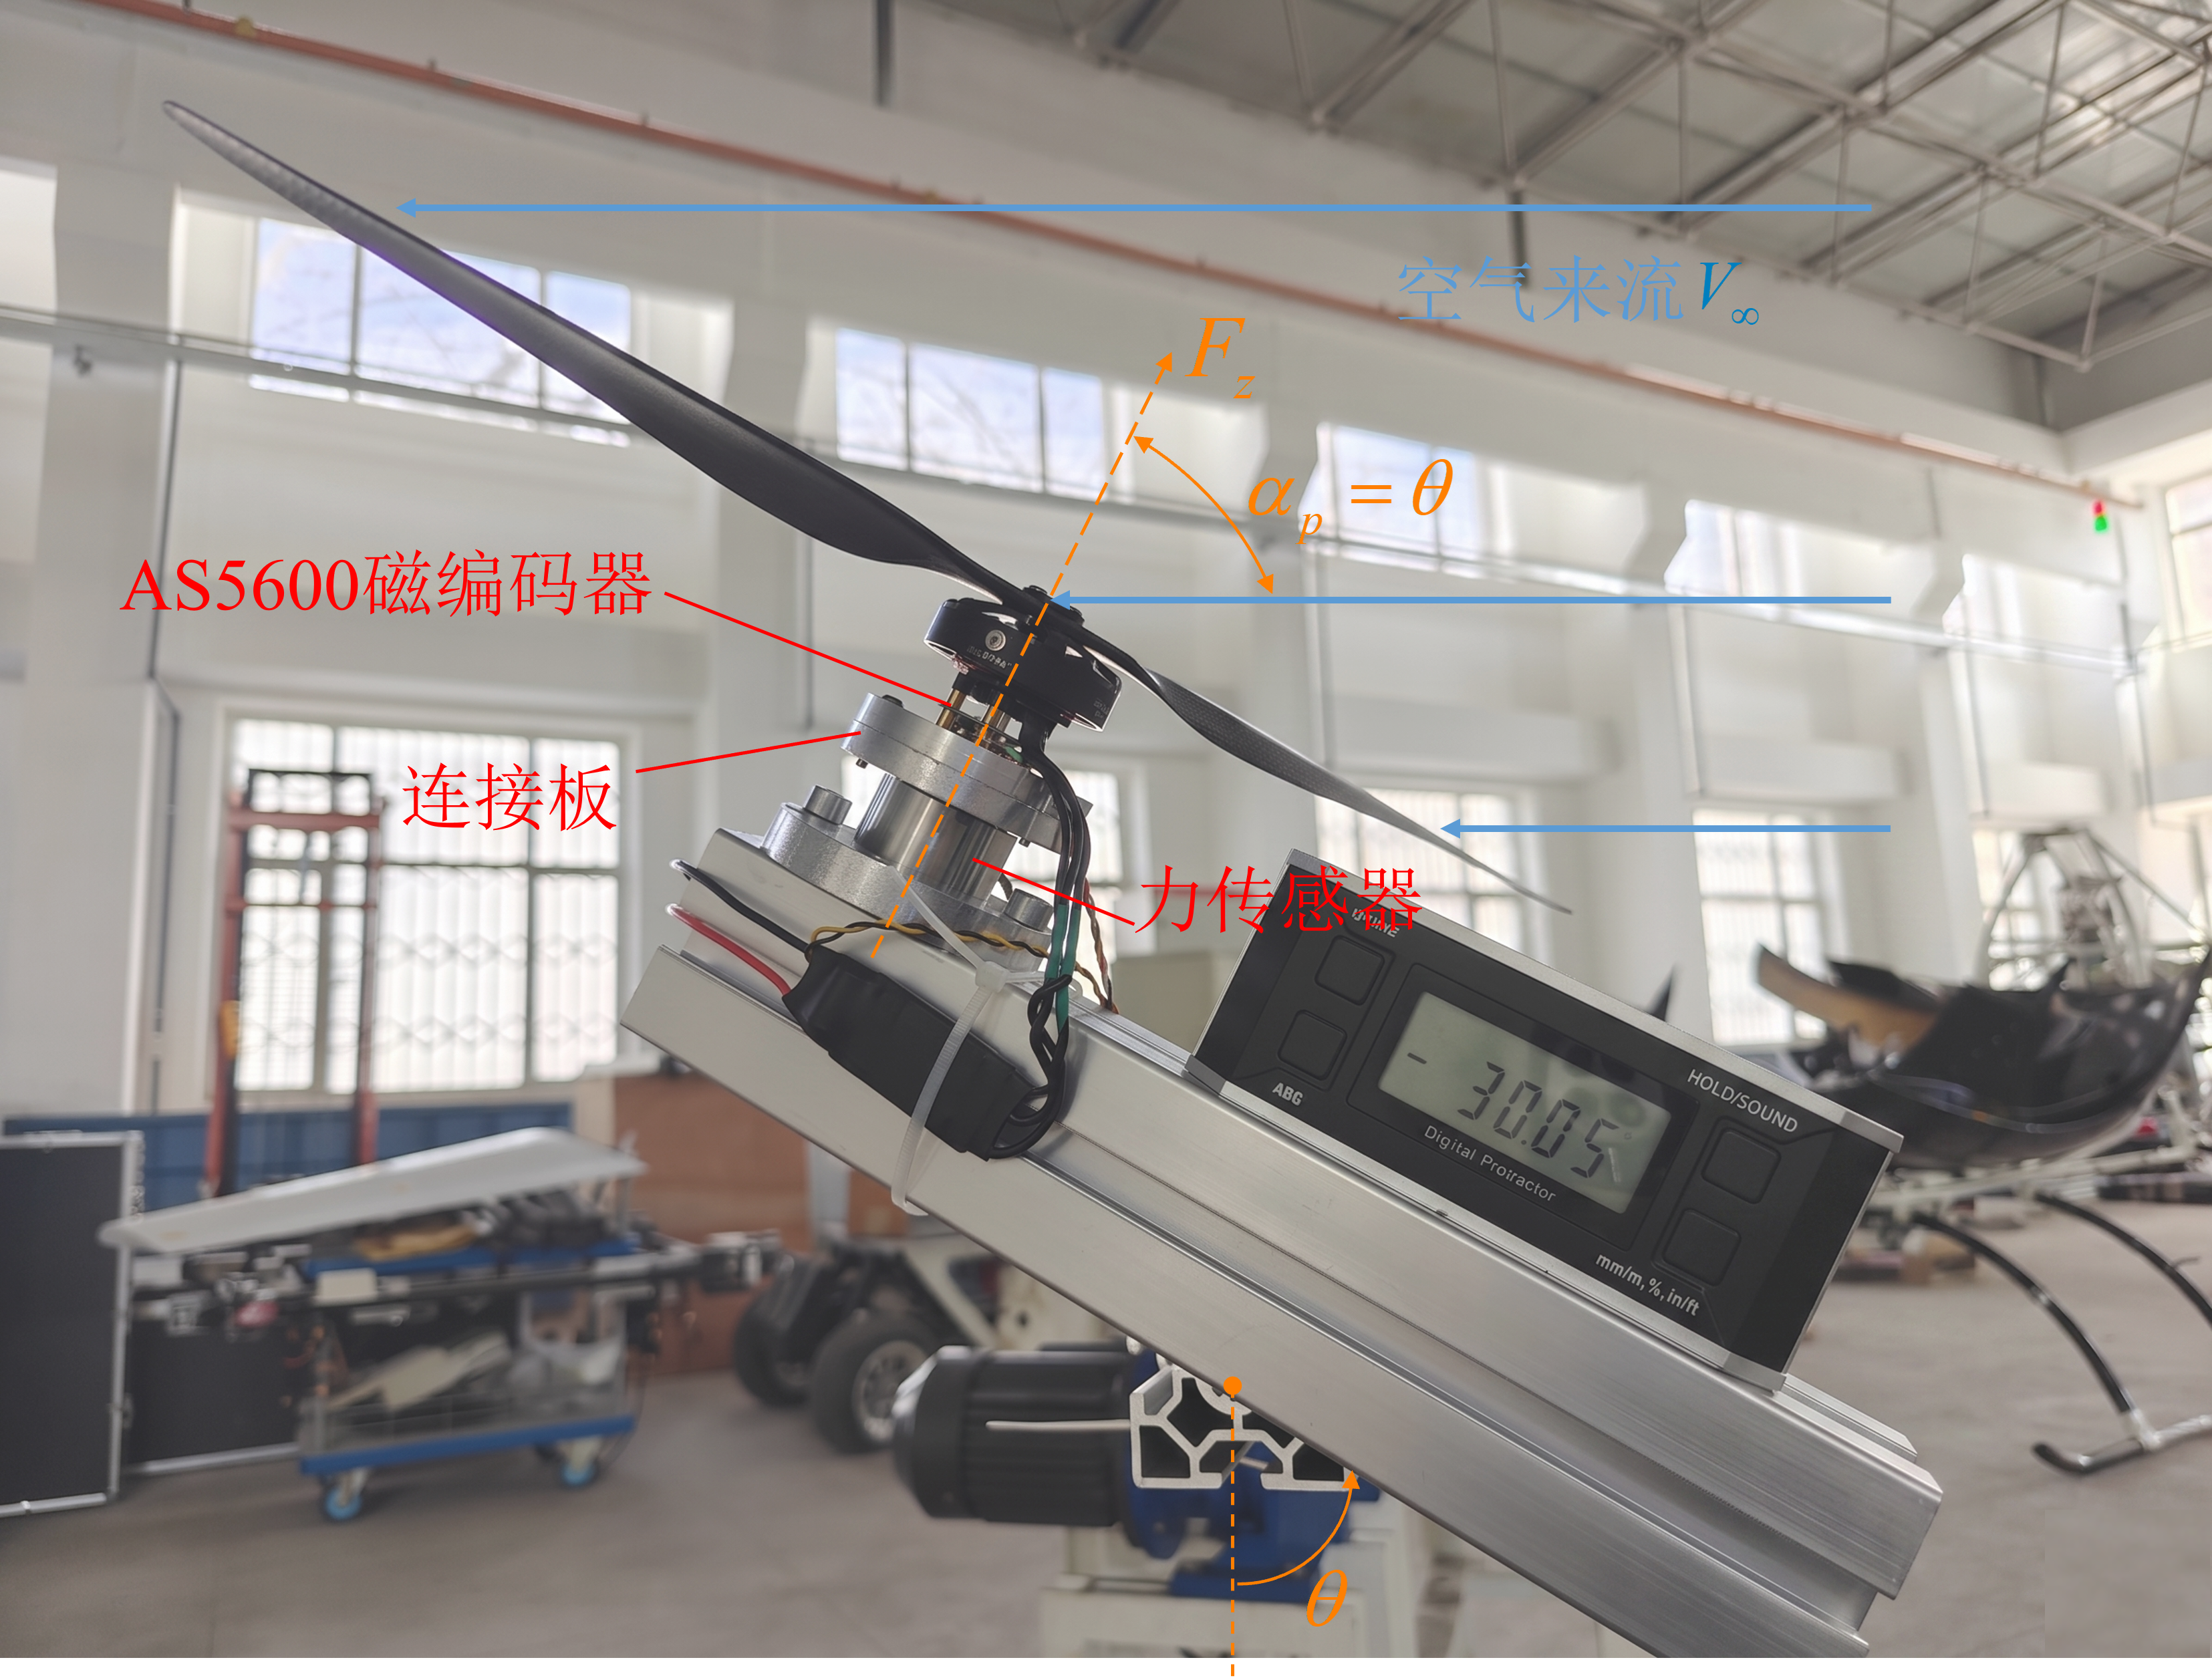
\includegraphics[width=8cm]{Image/图6b-旋转测试台.png}}
{\small (b)}
\vskip2mm
{\small 图6\quad 旋转悬臂式单旋翼测试平台;(a)整体结构;(b)旋翼单元
\\
Fig.\,6\quad Rotating cantilevered single-rotor test platform; (a) overall structure; (b) rotor unit}}
\end{center}

当$\alpha_p\neq0$时,旋翼单元中心的相对来流同时具有垂直于桨盘的轴向分量$V_{a,i}$和位于桨盘内的切向分量$V_{t,i}$:
\begin{equation}
V_{a,i}=\Omega_a R_0\cos\alpha_p,\qquad
V_{t,i}=\Omega_a R_0\sin\alpha_p
\label{eq:bench_map}
\end{equation}
代入式~(\ref{eq:mu_lambda})即可得到测试台工况下的前进比$\mu_i$与轴向入流比$\lambda_{c,i}$,进而由式~(\ref{eq:glauert})确定平均诱导入流比$\lambda_{\mathrm{ind},i}$.

桨叶坐标遵循图2定义,对位于$(\rho,\psi)$处的叶素,局部轴向速度$U_P$和切向速度$U_T$表示为:
\begin{equation}
\begin{aligned}
U_P(\rho,\psi)&=\Omega_a(R_0-\rho\cos\psi)\cos\alpha_p+v_{\mathrm{ind}}(\rho,\psi)\\
U_T(\rho,\psi)&=\Omega_a\rho-\Omega_a(R_0-\rho\cos\psi)\sin\alpha_p\cos\psi
\end{aligned}
\label{eq:bench_vel}
\end{equation}
式中,$v_{\mathrm{ind}}(\rho,\psi)$为诱导速度,由式~(\ref{eq:ind_vel})确定.由式~(\ref{eq:aoa})可得入流角$\phi$和叶素有效迎角$\alpha_{\mathrm{eff}}$.

旋翼测试台基本参数如表1所示,测试台能构造的最大来流速度为10.2m/s,根据$\tau=J\dot{\omega}$,带负载能达到的最大角加速度$\dot{\omega}$为7.38\,rad/s$^{2}$,旋翼单元受到指向旋转轴的向心过载最大为7.1g,受到的面向来流的过载最大为1.1g.

现有关于高机动飞行的研究中[4,19,20]最大速度的量级在5--12.9m/s,沿总升力方向的过载量级在1.63--2.2g.本文搭建的测试台能基本涵盖上述指标,因此能在式~(\ref{eq:state_aero})的变量层面和式~(\ref{eq:hub_a})的加速度层面构造高机动飞行下的动态来流.

\begin{center}
\vbox{\centering{\small 表1\quad 旋翼测试台参数
\\
Table\,1 \quad Rotor test bench parameters} \vskip2mm
{\footnotesize\centering
\begin{tabular}{cc}
\toprule
参数 & 值 \\
\midrule
总转动惯量 $J$ & 9.42\,kg$\cdot$m$^{2}$ \\
悬臂长度$R_0$ & 1.5\,m \\
最大转速$\Omega_{a,\max}$ & 64.9\,rpm \\
最大扭矩$\tau$ & 69.5\,N$\cdot$m \\
\bottomrule
\end{tabular}}}
\end{center}

\begin{center}
\begin{minipage}{0.98\columnwidth}
\centering
{\small 算法1\quad 离线升力查找表生成
\\
Algorithm\,1\quad Offline generation of the thrust lookup table}
\vskip2mm
\footnotesize
\begin{algorithmic}[1]
\Require 桨叶几何与翼型极线;工况网格 $\{\alpha_p,V_\infty,\Omega\}$
\Ensure 升力表 $T(\alpha_p,V_\infty,\Omega)$
\For{每个 $(\alpha_p,V_\infty)$}
    \State $V_a,\ V_t,\ \psi_w\gets V_\infty/\alpha_p$
    \For{每个 $\Omega$}
        \State 初始化诱导入流比 $\lambda_{\mathrm{ind}}$
        \Repeat
            \State 由式~(\ref{eq:bench_vel}) 计算局部来流速度
            \State 按式~(\ref{eq:dLdD})--(\ref{eq:dT}) 积分叶素升力 $T$
            \State 按式~(\ref{eq:glauert}) 阻尼更新 $\lambda_{\mathrm{ind}}$
        \Until{$\lambda_{\mathrm{ind}}$ 收敛或达到迭代上限}
        \State 存储 $T(\alpha_p,V_\infty,\Omega)$
    \EndFor
    \State 校验 $T$ 沿 $\Omega$ 方向单调递增
\EndFor
\end{algorithmic}
\end{minipage}
\end{center}

\subsection{飞控部署}
上述推导的完整叶素动量理论模型,计算量庞大,难以在机载控制器上实时求解.因此本文采用全工况离线求解、在线查表的部署方式:

1. 离线阶段在 $(\alpha_p,V_\infty,\Omega)$ 网格上求解正向升力模型并生成查找表,流程如算法1~所示;

2. 在线阶段依据期望升力与实时工况量反查所需转速(见算法2).

3. 在线查表给出期望升力到转速的前馈逆映射,而转速还需进一步转换为归一化电机控制量.在实际测试中,0-10\,m/s左右的来流下,转速-控制量之间的关系基本恒定,影响升力的是实际升力与转速之间的关系.为使前馈项的转速输出能够发挥作用,需要先标定转速-控制量之间的静态映射关系:在固定台架上选择0-100\%油门之间的13个固定点位,读取对应的电机控制量和实际转速,拟合得到
\begin{equation}
u_{\mathrm{ff}}=a\,\Omega^2+b\,\Omega+c
\label{eq:rpm_calib}
\end{equation}
其中,$\Omega$ 为电机转速,$a,b,c$ 为拟合出的常系数.

4. 反馈补偿器选用 PID 控制器,其结构简单、计算量小,能够以较高频率运行以快速抑制模型残差与外部扰动.
\begin{center}
\begin{minipage}{0.98\columnwidth}
\centering
{\small 算法2\quad 在线升力逆查表
\\
Algorithm\,2\quad Online inverse lookup of the thrust table}
\vskip2mm
\footnotesize
\begin{algorithmic}[1]
\Require $T_c$、$\Omega_a$、$\alpha_p$、$R_0$;离线升力表 $T$
\Ensure 前馈转速 $\Omega_{\mathrm{ff}}$
\State $V_\infty\gets\Omega_aR_0$
\State 将 $(\alpha_p,V_\infty)$ 限制在表内并双线性插值得 $T(\Omega_k)$
\State $T_c^*\gets\operatorname{clip}\!\left(T_c,T(\Omega_0),T(\Omega_{K-1})\right)$
\State 沿 $\Omega$ 方向反插 $\Omega_{\mathrm{ff}}\gets T^{-1}(T_c^*)$
\State \textbf{return}\ $\Omega_{\mathrm{ff}}$
\end{algorithmic}
\end{minipage}
\end{center}

\subsection{力传感器集成}
直接升力反馈要求传感器能够在不改变主要传力路径的条件下测量旋翼轴向作用力.应变片机臂测力方案易受结构模态、温漂与装配差异影响,而专用力传感器能够提供更直接的载荷观测[6,13].本文采用SBT673小型拉压力传感器,额定量程为10kg,对应额定轴向力为98.07N,标称精度为0.1$\%$.

如图6(b)所示,测量组件自上而下依次由螺旋桨、电机、连接板、力传感器组成.螺旋桨产生的轴向升力经电机与连接板传递至传感器受力端.传感器信号经零偏校准、比例换算和低通滤波后得到升力测量值$T_i$.

所述零偏校准,主要用于补偿传感器安装载荷在轴向和径向过载工况下产生的测量误差.具体而言，当旋翼电机无转速时，在旋转测试台上，进行不同加速时间(测试台从静止到最大转速的时间)的动态测试，补偿后的输出模型为:
\begin{equation}
\hat{T}_i=T_i-A\,a_z-B\,a_x
\label{eq:sensor_calib}
\end{equation}
其中$\hat{T}_i$为补偿后的传感器测量值,单位为N;$A$=0.361、$B$=0.033,分别为传感器轴向和径向载荷的补偿系数,与传感器安装的载荷质量与安装误差有关,单位为kg;$a_z$和$a_x$分别为沿传感器轴向和径向的加速度值,通过测试台悬臂末端安装的飞控加速度计获取,并投影到传感器轴向和径向,单位为m/s².补偿前后的传感器测量数据如图7所示.

\section{结果}
\label{sec:experiment}

为验证所提出的旋翼升力模型与升力闭环控制器,本文在旋转测试台上开展两类实验:其一,执行如表2所示的工况测试,将第1节叶素动量模型的预测升力与实测升力对比,验证模型精度;其二,按传统升力开环控制、纯升力反馈、模型前馈与升力反馈复合控制三级对照方案,验证所提出的升力反馈和前馈-反馈复合控制方案的控制效果.

\subsection{旋翼升力模型精度验证}
\label{subsec:model_verif}
测试对象为T-Motor MN5008 KV340电机与P18$\times$6.1\,CF螺旋桨,旋翼轴向升力由同轴力传感器测量,转台角速度由安装在悬臂末端的飞控惯性测量单元(IMU)记录,电机转速由AS5600磁编码器获取.试验选取约3000、4000和5000\,rpm的典型转速,在每个工况点停留3s,记录对应的旋翼转速和升力,具体实验设置如表2所示.

\begin{center}
\vbox{\centering{\small 表2\quad 旋翼测试台测试设置
\\
Table\,2 \quad Test settings of the rotor test bench} \vskip2mm
{\footnotesize\centering
\begin{tabular}{ccc}
\toprule
转速档位 & 攻角 & 来流速度 \\
\midrule
3000\,rpm & \multirow{3}{*}{0-90$^{\circ}$(间隔15$^{\circ}$)} & \multirow{3}{*}{0-10.2\,m/s(间隔10\%)} \\
4000\,rpm & & \\
5000\,rpm & & \\
\bottomrule
\end{tabular}}}
\end{center}

设置3组转速档位、7种不同攻角、11个来流速度,共231个分档工况点,每个工况点以式~(\ref{eq:mu_lambda})定义的螺旋桨前进比表示.以式~(\ref{eq:glauert})定义的升力系数$C_{T}$作为精度衡量指标.定义相对误差为实测值$\delta C_T=C_{T,\mathrm{exp}}$与理论值$C_{T,\mathrm{theory}}$之差,正值对应模型低估,负值对应模型高估.分攻角进行统计,采用归一化均方根误差(NRMSE)、归一化最大绝对误差和平均绝对百分比误差(MAPE)评价模型精度.前两项指标分别将升力系数的均方根误差和最大绝对误差除以对应统计组的实测升力系数均值;MAPE则为各工况相对误差绝对值的算术平均.
\begin{center}
\vbox{\centering
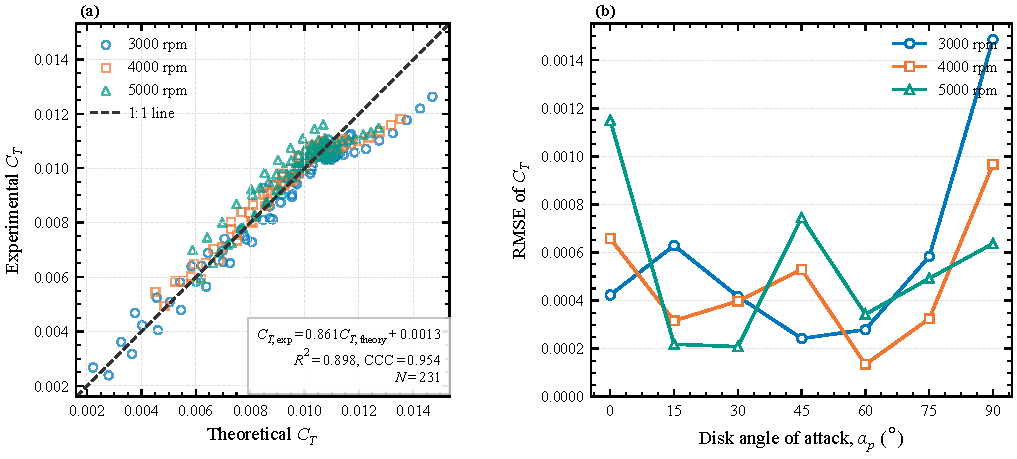
\includegraphics[width=7.5cm]{Image/fig9_rotor_model_diagnostics.pdf}\\[1mm]
{\small 图7\quad 升力系数一致性与攻角分区相对误差分布
\\ Fig.\,7 \quad Thrust coefficient agreement and relative-error distributions by disk angle of attack}
}
\end{center}

图7(a)给出了理论与实测升力系数的对比.三个转速档位的散点总体沿1:1参考线分布,85.28$\%$的工况位于±10$\%$相对误差带内,表明模型在所测转速和来流范围内具有较好的升力预测能力.较高理论升力系数区域的部分散点偏离参考线并位于其下方,说明模型在部分工况下仍存在高估,预测精度在整个试验包线内非均匀分布。

图7(b)进一步展示了不同桨盘攻角下的相对误差分布.0°和45°组的误差中位数为正,模型总体偏向低估;75°和90°组则为负,模型总体偏向高估,其中90°组的负偏差更为明显.相比之下30°和60°组的误差分布更接近零值.上述结果表明,$\delta C_T=C_{T,\mathrm{exp}}$--$C_{T,\mathrm{theory}}$残差随来流方向发生变化,具有工况依赖性;需要结合全部工况的总体误差与分攻角误差结果,才能完整反映模型的适用范围.

\begin{center}
\vbox{\centering{\small 表3\quad 不同桨盘攻角下的旋翼升力模型误差统计
\\ Table\,3 \quad Error statistics of the rotor lift model at different disk angles of attack}\vskip2mm
{\scriptsize\centering
\setlength{\tabcolsep}{3.5pt}
\begin{tabular}{@{}crrr@{}}
\toprule
$\alpha_p/(^\circ)$ & NRMSE/\% & MaxErr$_{\mathrm{norm}}$/\% & MAPE/\% \\
\midrule
0 & 9.43 & 15.82 & 8.51 \\
15 & 4.92 & 10.18 & 4.83 \\
30 & 3.43 & 10.91 & 2.98 \\
45 & 5.77 & 10.02 & 5.12 \\
60 & 2.65 & 7.38 & 2.15 \\
75 & 4.16 & 7.12 & 3.67 \\
90 & 10.13 & 18.79 & 8.03 \\
全部 & 6.56 & 22.18 & 5.04 \\
\bottomrule
\end{tabular}}
}
\end{center}

表3汇总了总体及分攻角误差。全部工况的NRMSE为6.56$\%$，MAPE为5.04$\%$，说明模型整体的预测精度较高。在15°—75°斜来流范围内，分攻角NRMSE为2.65$\%$—5.77$\%$；0°和90°工况的NRMSE分别为9.43$\%$和10.13$\%$，均高于中间攻角组。结合图7可知，模型在所测斜来流范围内保持了较好的预测精度，而在纯轴向和纯侧向来流两个端点工况下仍存在较明显的偏差。

其他关于叶素动量理论(BEMT)旋翼建模的研究中,误差量级为:Carroll[18]等使用激光扫描提取桨叶翼型和气动参数,建立了与本文一致的TmotorP18$\times$6.1螺旋桨的变攻角BEMT模型,其理论与试验结果的误差范围为$5\%-15\%$;Serrano等[9]表明,引入Glauert或Coleman非均匀入流模型后,非零攻角下的最大偏差可控制在$15\%$以内;Theys等[8]则指出,传统BEMT和涡格法虽能预测斜流下的总体趋势,但精度会随来流倾斜显著下降,在小角度下误差量级约为$10\%$,在大角度斜流下误差量级约$10\%-30\%$.相比之下,本文模型在各攻角下的RMSE小于$10.5\%$,在所有工况点下的最大误差小于$20\%$,与现有研究中的旋翼模型精度处于同一量级,进一步验证了\ref{subsec:geo}节中摄影测量的精度和旋翼叶素模型的准确性.该精度能够为后续模型前馈提供有效基准,其余模型失配则由升力反馈进一步补偿.
\begin{center}
\vbox{\centering
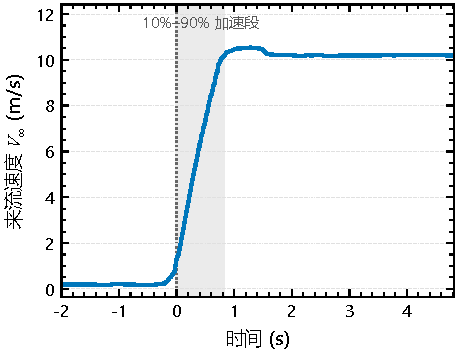
\includegraphics[width=8cm,height=3.8cm]{Image/fig9_freestream_ramp.pdf}\\[1mm]
{\small 图8\quad 来流速度曲线
\\ Fig.\,8 \quad Freestream-speed curve }}
\end{center}

\subsection{升力闭环控制效果验证}
\label{subsec:control_verif}

本节以0$^{\circ}$攻角下的纯轴向来流作为控制验证工况:该工况下来流方向垂直于桨盘平面、轴向分量最大,对旋翼升力的扰动最直接,因此适合用于检验控制器对显著气动扰动的抑制能力.进行三级对照实验:

1. 固定控制量方案按式~(\ref{eq:static_map})根据零来流静态标定关系给定与期望升力对应的控制量,并在来流变化期间保持不变;

2. 纯反馈方案关闭第2.2节所述的旋翼升力模型前馈,仅由升力误差生成反馈修正量$u_{\mathrm{fb}}$;

3. 模型前馈与反馈复合控制依据转台角速度$\Omega_a$与桨盘攻角$\alpha_p$估计的来流状态,通过旋翼升力逆模型及转速--控制量映射生成前馈控制量$u_{\mathrm{ff}}$,叠加反馈修正量$u_{\mathrm{fb}}$得到总输出$u_{\mathrm{c}}$;$u_{\mathrm{ff}}$和$u_{\mathrm{fb}}$直接相加,系数均为1,其实际贡献随工况和跟踪误差变化.

\end{multicols}
\begin{center}
\vbox{\centering
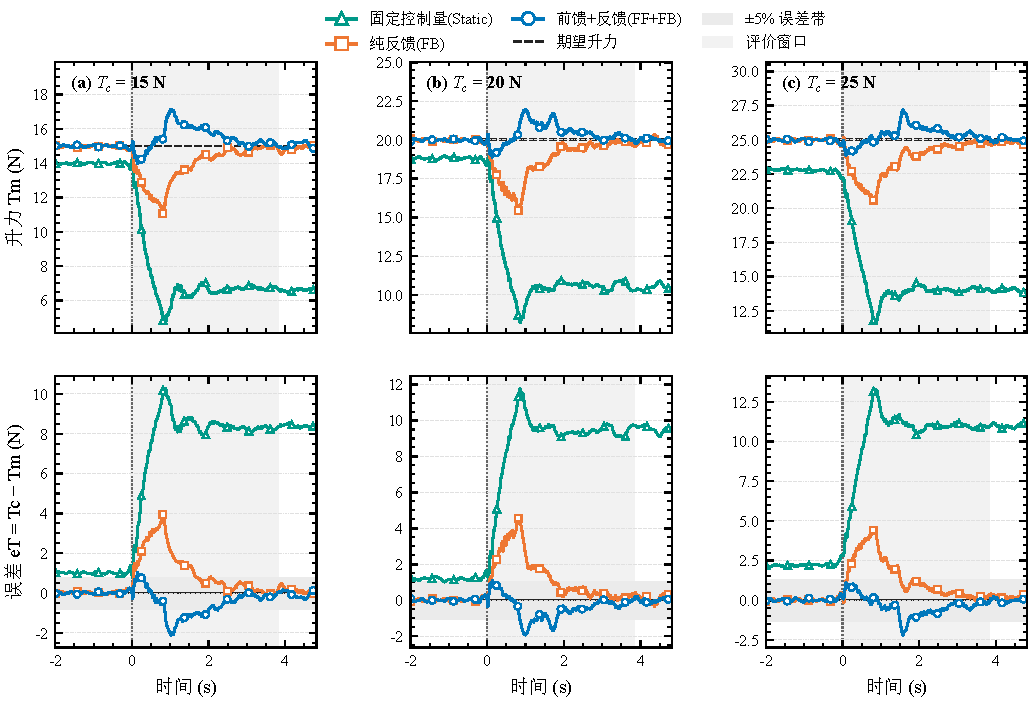
\includegraphics[width=15.5cm]{Image/fig10_representative_response.pdf}\\[1mm]
{\small 图9\quad 15、20、25 N期望升力和1 s来流加速工况下三种控制方法的动态响应.(a)--(c)分别为15、20、25 N期望升力下的实测升力与跟踪误差.
\\ Fig.\,9 \quad Dynamic response of the three control methods under 15, 20, and 25\,N desired thrust with the 1\,s freestream-acceleration condition. (a)--(c) show the measured thrust and tracking error under 15, 20, and 25\,N desired thrust, respectively.}}
\end{center}
\begin{multicols}{2}

其中,纯升力反馈方案与复合控制方案采用相同的PID参数.试验覆盖15、20、25 N三中期望升力与1、5、10 s三种来流加速时间(测试台从静止到最大速度的时间),共9个工况;同一工况下三种方法在采用相同的目标升力阶跃指令、限幅及数据处理流程.

来流速度由转台角速度计算,即$V_\infty=\Omega_a R_0$.图8给出三种加速过程及时间对齐方式,根据中值滤波后的$V_\infty$,将其达到低、高平台速度增量10\%和90\%的时刻分别记为$t_{10}$和$t_{90}$,评价窗口统一取$[t_{10},t_{90}+3,\mathrm{s}]$,包含主要加速过程及其后的恢复阶段.图9和图10沿用这一对齐规则;图中的纵向阴影标示10\%—90\%加速段,水平阴影标示期望升力的±5\%误差带.以$e_T=T_c-T_m$定义升力跟踪误差，并采用期望升力归一化的均方根误差评价控制效果.

图9比较1 s快速来流条件下不同期望升力的动态响应.三种期望升力下,固定控制量方案均随来流增强出现明显的升力下降,且来流稳定后仍不能恢复至目标值,表明零来流下的静态映射难以适应轴向来流变化.纯反馈能够恢复升力,但加速阶段存在较大的瞬态跌落,体现出依赖升力偏差建立补偿的响应局限.复合控制则减小了这一跌落,但在随后恢复过程中仍有一定超调.因此,前馈的作用主要体现为减轻来流变化过程中的升力偏离,而非完全消除瞬态误差.(最后一句再润色)
\end{multicols}
\begin{center}
\vbox{\centering
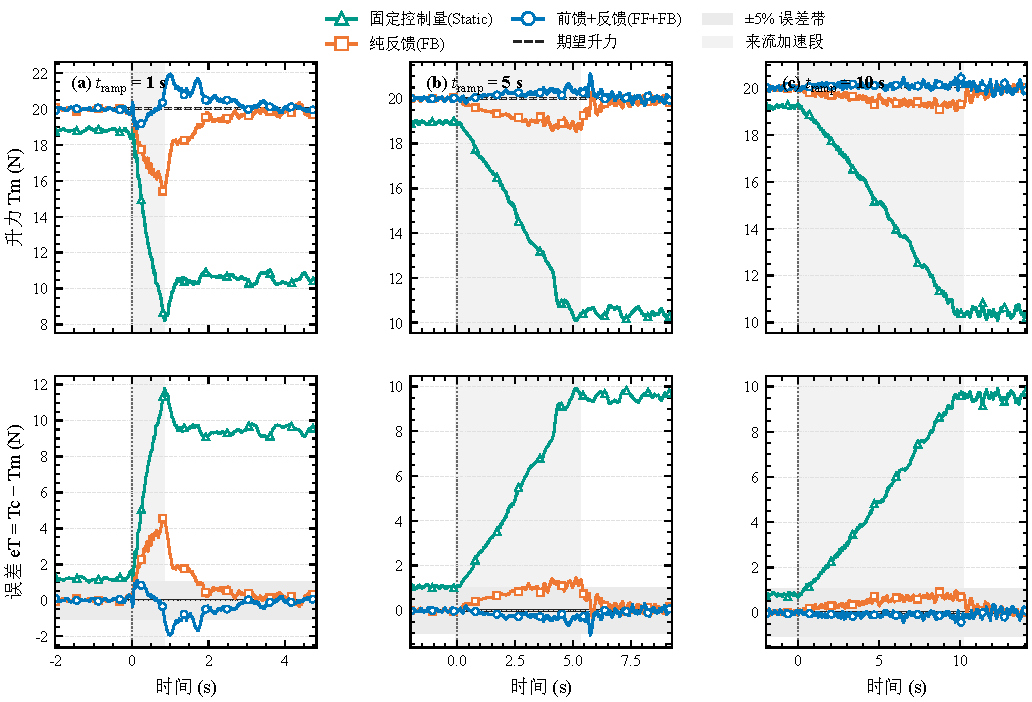
\includegraphics[width=14cm]{Image/fig10_ramp_time_response_20N.pdf}\\[1mm]
{\small 图10\quad 1、5、10 s来流加速时间下20N期望升力的三种控制方法的动态响应.(a)--(c)分别为1、5、10 s加速时间下的实测升力变化曲线与跟踪误差.
\\ Fig.\,10 \quad Dynamic response of the three control methods under 20\,N desired thrust with the 1, 5, and 10\,s freestream-acceleration conditions. (a)--(c) show the measured thrust and tracking error under the 1, 5, and 10\,s acceleration times, respectively.}}
\end{center}
\begin{multicols}{2}

\begin{center}
\vbox{\centering{\small 表4\quad 统一扰动窗口下9种期望升力--加速时间组合的归一化RMSE及降幅
\\ Table\,4 \quad Normalized RMSE and reduction ratios for the 9 desired-thrust/acceleration-time combinations using a common disturbance-window definition}\vskip2mm
{\scriptsize\centering
\setlength{\tabcolsep}{1.8pt}%
\begin{tabular}{@{}ccccccc@{}}
\toprule
$T_c$/N & $t_{\mathrm{ramp}}$/s & Static/\% & FB/\% & FF+FB/\% & FB降幅/\% & FF+FB降幅/\% \\
\midrule
15 & 1  & 54.13 & 10.39 & 5.64 & 80.8 & 45.7 \\
15 & 5  & 44.62 & 4.61  & 2.42 & 89.7 & 47.5 \\
15 & 10 & 39.43 & 3.02  & 1.27 & 92.3 & 57.8 \\
20 & 1  & 45.75 & 9.06  & 3.87 & 80.2 & 57.3 \\
20 & 5  & 37.58 & 3.99  & 1.44 & 89.4 & 63.9 \\
20 & 10 & 33.82 & 2.65  & 0.76 & 92.2 & 71.4 \\
25 & 1  & 42.65 & 7.67  & 2.90 & 82.0 & 62.2 \\
25 & 5  & 35.91 & 3.54  & 1.21 & 90.1 & 65.8 \\
25 & 10 & 32.73 & 2.32  & 0.60 & 92.9 & 74.3 \\
\bottomrule
\end{tabular}}
\vskip1mm
{\scriptsize\raggedright 注:三种方法的NRMSE均以$T_c$归一化,窗口均为$[t_{10},t_{90}+3\,\mathrm{s}]$.FB降幅相对固定控制量,FF+FB降幅相对纯反馈.\par}
}
\end{center}

图10进一步比较20 N期望升力下不同来流加速时间的响应.随着加速时间延长,纯反馈的瞬态偏差减小,说明较缓的来流变化为反馈调节提供了更充分的响应时间;相比之下,固定控制量方案在来流稳定后仍保留较大的升力亏损,表明减缓来流变化不能消除静态映射失配.复合控制在三种加速时间下均保持较小的跟踪偏差,其中1 s工况更清楚地呈现了对瞬态跌落的抑制效果.

表4汇总全部9个工况的误差指标。纯反馈相对固定控制量的NRMSE降低80.2\%—92.9\%；加入模型前馈后，相对纯反馈进一步降低45.7\%—74.3\%，复合控制的NRMSE为0.60\%—5.64\%。全部所测工况均呈现相同的误差排序$E_{\mathrm{FF+FB}}<E_{\mathrm{FB}}<E_{\mathrm{static}}$，说明升力反馈能够补偿静态映射失配，模型前馈则在此基础上进一步改善跟踪性能。
\begin{center}
\vbox{
\centerline{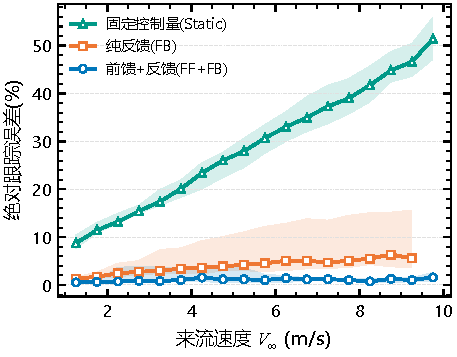
\includegraphics[width=8cm,height=5.5cm]{Image/fig12_speed_error.pdf}}
\vskip2mm
{\small 图11\quad 三种控制方法归一化绝对误差随来流速度的变化
\\ Fig.\,11 \quad Normalized absolute tracking error of the three control methods over the freestream-speed sweep}}
\end{center}


图11从来流速度维度补充上述窗口统计结果，给出9个工况归一化绝对误差$|e_T|/T_c$的中位数及四分位区间。随着来流速度增大，固定控制量方案的误差明显增加；纯反馈显著降低了误差，但仍存在一定的工况间差异；复合控制的误差中位数总体维持在较低水平，四分位区间也较窄。这表明其改善作用在所测不同期望升力和加速时间下具有一致性。

为解释前馈的补偿过程，图12以20 N／1 s工况为例，选取纯反馈试验和复合控制试验，依次给出控制输出及转速响应。两次试验分别以自身来流的$t_{10}$对齐，随着来流增大，逆模型给出的前馈参考转速上升，并经式~(\ref{eq:rpm_calib})静态映射直接提高前馈控制量。复合控制的反馈项在加速阶段提供正向修正，随后随升力超调转为负向修正，体现了反馈对剩余偏差的补偿作用。纯反馈则由PID根据已产生的升力偏差建立全部控制输出。

转速对照以两种方法各自的扰动前、后平台确定转速增量，其达到50\%增量的相对时刻分别约为0.277 s和0.415 s，即复合控制提前约0.14 s。上述时刻由原始采样序列首次越阈确定，保留实测波动，不能将其解释为统一的相位或传输延迟。在相同PID参数下，图9(b)和表4显示该工况的升力NRMSE由9.06\%降至3.87\%，降低57.3\%。控制量分解、实测转速和升力误差共同支持以下解释：模型前馈利用当前来流信息直接建立补偿，升力反馈进一步修正模型失配与动态偏差，从而减轻纯反馈补偿建立过程中产生的瞬态升力损失。

\begin{center}
\vbox{
\centerline{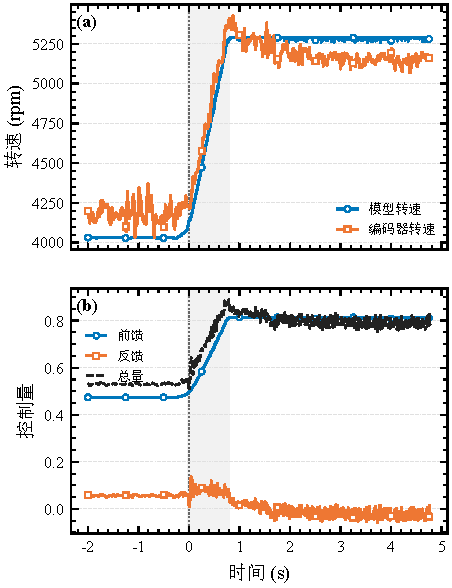
\includegraphics[width=8cm]{Image/fig13_feedforward_mechanism.pdf}}
\vskip2mm
{\small 图12\quad 20 N期望升力、1 s来流加速工况下的前馈补偿过程：(a)两种方法的总控制输出及复合控制的前馈、反馈分量；(b)两种方法的实测转速与复合控制的前馈参考转速。两次试验分别以各自来流达到10\%增量的时刻对齐。灰色阴影为10\%—90\%加速段，两幅子图统一采用FF+FB试验的边界，$\tau\in[0,0.791]$ s。
\\ Fig.\,12 \quad Feedforward compensation at a desired thrust of 20 N with a 1 s inflow acceleration time: (a) total control outputs and the feedforward and feedback components of combined control; (b) measured rotor speeds and the feedforward rotor-speed reference. Each trial is aligned at its own 10\% inflow-increment instant. Gray shading indicates the 10\%--90\% acceleration segment; both panels use the FF+FB trial boundaries, $\tau\in[0,0.791]$ s.}
\vskip1mm
{\scriptsize\raggedright 注：(a)比较日志中同一控制器叠加节点的归一化输出，不代表最终PWM输出。加速段阴影不同于完整评价窗口$[t_{10},t_{90}+3\,\mathrm{s}]$。实测转速保留全部原始采样点。\par}}
\end{center}

\section{结论}

本文针对多旋翼无人机机动飞行中的推进系统升力失配问题,建立了从整机运动状态到单旋翼轴向升力的机理模型,并提出基于模型前馈与直接力反馈的升力闭环控制方法.模型未使用升力试验数据拟合气动参数或修正升力预测值,但仍依赖桨叶几何获取与标定、XFOIL数值极线以及转速--控制量静态标定.在已测试的模型验证包线内,总体归一化RMSE为5.76\%,在$15^{\circ}$--$75^{\circ}$斜来流范围内,按攻角汇总的归一化RMSE为2.46\%--5.02\%.

控制效果的验证层级为执行器层单旋翼,适用范围限定为本文所测$\alpha_p=0^{\circ}$的轴向强来流工况.在15、20、25 N期望升力与1、5、10 s加速时间构成的9个工况中,按统一扰动窗口及期望升力归一化,纯反馈相对固定控制量的RMSE降低80.2\%--92.9\%,前馈与反馈复合控制相对纯反馈进一步降低45.7\%--74.3\%,其NRMSE为0.60\%--5.64\%.在20 N/1 s代表工况中,复合控制实测转速达到50\%增量的时刻较纯反馈提前约0.14 s,与该工况升力NRMSE降低57.3\%的结果共同体现了前馈的扰动补偿作用.上述结果量化了模型前馈在轴向强来流下对单旋翼升力跟踪的改善,尚不能直接外推为斜来流控制效果或整机姿态、轨迹控制的端到端收益.

未来工作包括:1) 轻量化旋翼测量单元,使其能够集成到多旋翼无人机结构中;2) 补充不同斜来流攻角下的闭环扰动试验,检验前馈通道对来流方向变化的补偿能力;3) 在旋翼悬臂式旋转测试台末端安装可进行姿态控制的双旋翼单元或四旋翼整机,并结合整机飞行试验,验证姿态、轨迹跟踪及控制分配的端到端收益.

\begin{thebibliography}{99}
\zihao{6} \addtolength{\itemsep}{0.2em} \urlstyle{rm}

\bibitem{1} 王姣娥, 杜德林, 陈卓, 黄洁, 张兵, 莫辉辉, 等. 中国低空经济发展指数报告(2026). 北京: 中国科学院地理科学与资源研究所, 2026

\bibitem{2} Chen Lin, Miao Zhi-Qiang, Wang Xiang-Ke, Chen Mou, Duan Hai-Bin, Wang Yao-Nan. Overview on autonomous aircraft technology and its application to low-altitude economy. {\sl Robot}, 2025, {\bf 47}(3): 470$-$496 \\
(陈林, 缪志强, 王祥科, 陈谋, 段海滨, 王耀南. 自主飞行器技术及其在低空经济中的应用综述. 机器人, 2025, 47(3): 470$-$496)

\bibitem{3} Bauersfeld L, Kaufmann E, Foehn P, Sun S, Scaramuzza D. NeuroBEM: Hybrid aerodynamic quadrotor model. In: Proceedings of Robotics: Science and Systems XVII (RSS). Virtual: RSS Foundation, 2021

\bibitem{4} Liu H, Lin D, Ye J, Jiang T, Huang J S. Quadrotor aggressive control based on angular acceleration feedback and high-fidelity propulsion model. {\sl IEEE Transactions on Industrial Electronics}, DOI: 10.1109/TIE.2025.3572921

\bibitem{5} Gonzalez-Morgado A, Sanchez-Cuevas P J, Heredia G, Ollero A. Rotor-force controller for multirotors under aerodynamic interferences. {\sl Aerospace Science and Technology}, 2025, {\bf 157}: 109861

\bibitem{6} Jiang Han, Chang Yan-Chun, Yang Li-Ying, He Yu-Qing. Thrust feedback-based control method for rotor UAV. {\sl Robot}, 2026, {\bf 48}(3): 518$-$530 \\
(蒋涵, 常彦春, 杨丽英, 何玉庆. 基于升力反馈的旋翼无人机控制方法. 机器人, 2026, 48(3): 518$-$530)

\bibitem{7} Jiang Han, Chen Ze-Hao, Chang Yan-Chun, Yang Li-Ying, Liu Lian-Qing, He Yu-Qing. A wind disturbance suppression method for multirotor UAVs based on direct thrust control. {\sl SCIENTIA SINICA Technologica}, 2026, {\bf 56}, DOI: 10.1360/SST-2025-0274 \\
(蒋涵, 陈泽昊, 常彦春, 杨丽英, 刘连庆, 何玉庆. 基于直接升力控制的旋翼无人机风扰抑制方法. 中国科学: 技术科学, 2026, 56, DOI: 10.1360/SST-2025-0274)

\bibitem{8} Theys B, Dimitriadis G, Hendrick P, De Schutter J. Experimental and numerical study of micro-aerial-vehicle propeller performance in oblique flow. {\sl Journal of Aircraft}, 2017, {\bf 54}(3): 1076$-$1084

\bibitem{9} Serrano D, Ren M, Qureshi A J, Ghaemi S. Effect of disk angle-of-attack on aerodynamic performance of small propellers. {\sl Aerospace Science and Technology}, 2019, {\bf 92}: 901$-$914

\bibitem{10} Simmons B M. System identification for propellers at high incidence angles. {\sl Journal of Aircraft}, 2021, {\bf 58}(6): 1336$-$1350

\bibitem{11} Glauert H. A general theory of the autogyro. R\&M No. 1111. London: British Aeronautical Research Committee, 1926

\bibitem{12} Drela M. XFOIL: An analysis and design system for low Reynolds number airfoils. In: {\sl Low Reynolds Number Aerodynamics}. Berlin: Springer, 1989. 1$-$12

\bibitem{13} Meier L, Honegger D, Pollefeys M. PX4: A node-based multithreaded open source robotics framework for deeply embedded platforms. In: Proceedings of 2015 IEEE International Conference on Robotics and Automation (ICRA). Seattle, WA, USA: IEEE, 2015. 6235$-$6240

\bibitem{14} Selig M S. UIUC airfoil data site. Urbana-Champaign: University of Illinois at Urbana-Champaign. \url{https://m-selig.ae.illinois.edu/ads.html}

\bibitem{15} Tang E, Chung S J. Rapid extraction of propeller geometry using photogrammetry. {\sl International Journal of Micro Air Vehicles}, 2022, {\bf 14}: 1$-$22. DOI: 10.1177/17568293221132044

\bibitem{16} Baltsavias E P. A comparison between photogrammetry and laser scanning. {\sl ISPRS Journal of Photogrammetry and Remote Sensing}, 1999, {\bf 54}(2$-$3): 83$-$94. DOI: 10.1016/S0924-2716(99)00014-3

\bibitem{17} Cheng Z, Li H, Asano Y, Zheng Y, Sato I. Multi-view 3D reconstruction of a texture-less smooth surface of unknown generic reflectance. In: Proceedings of the IEEE/CVF Conference on Computer Vision and Pattern Recognition (CVPR). Virtual: IEEE, 2021. 16226$-$16235

\bibitem{18} Carroll T B. A design methodology for rotors of small multirotor vehicles [Master thesis]. Toronto, Canada: Ryerson University, 2017

\bibitem{19} Tal E, Karaman S. Accurate tracking of aggressive quadrotor trajectories using incremental nonlinear dynamic inversion and differential flatness. {\sl IEEE Transactions on Control Systems Technology}, 2021, {\bf 29}(3): 1203$-$1218

\bibitem{20} Wang M, Wang Q, Wang Z, Gao Y, Wang J, Cui C, et al. Unlocking aerobatic potential of quadcopters: Autonomous freestyle flight generation and execution. {\sl Science Robotics}, 2025, {\bf 10}: eadp9905

\end{thebibliography}

% TODO: 请作者填写作者简介(姓名、职称、学习工作经历、研究方向)与照片
\begin{biographynophoto}
\noindent{\hei 【待填写作者姓名】}\quad 【待填写作者简介】.\\E-mail: 【待填写邮箱】

\noindent({\bf 【待填写英文作者姓名】}\quad 【待填写英文作者简介】.)
\end{biographynophoto}

\end{multicols}
\end{document}
